\documentclass[11pt]{article}

\usepackage[margin=1in]{geometry}
\usepackage{setspace}
\onehalfspacing
\usepackage{graphicx}
\graphicspath{report_images/}
\usepackage{appendix}
\usepackage{listings}
\usepackage{float}
\usepackage{multirow}
\usepackage{amsthm}
% The next three lines make the table and figure numbers also include section number
\usepackage{chngcntr}
\counterwithin{table}{section}
\counterwithin{figure}{section}
% Needed to make titling page without a page number
\usepackage{titling}

% DOCUMENT INFORMATION =================================================
\font\titleFont=cmr12 at 11pt
\title {{\titleFont ECEN 429: Introduction to Digital Systems Design Laboratory \\ North Carolina Agricultural and Technical State University \\ Department of Electrical and Computer Engineering}} % Declare Title
\author{\titleFont Reporter: Chris Cannon \\ \titleFont Partner: Nikiyah Beulah} % Declare authors
\date{\titleFont April 5, 2018}
% ======================================================================

\begin{document}

\begin{titlingpage}
\maketitle
\begin{center}
	Lab 9
\end{center}
\end{titlingpage}

\section{Introduction}
This lab had us use finite state machines to implement traffic control systems. We used different sensors and logic in each part and had to adjust our finite state machines accordingly. This challenge is useful and practical because it we solved real world problems that we all experience every day with the skills we learned in this lab.

\section{Background, Design Solution, and Results}

\subsection{Problem 1 }

\subsubsection{Background}
Problem 1 requires a basic traffic control system that will start with North and South green, and will switch to East and West green when a vehicle arrives from the East or West. After allowing cars to travel East and West, the turn lane from the North will be allowed to turn before the South light turns green.

\subsubsection{Design Solution}
We used the clock divider developed in Lab 6 to help make this unit testable. We displayed our current count on a seven-segment display. We used a temporary count signal that will count up or down and then will be translated to the seven-segment display. The input ports are summarized in Table ~\ref{tab:counter_input_Ports} and the output ports are summarized in Table ~\ref{tab:counter_output_Ports}.

\begin{table}[H]
\begin{center}
\begin{tabular}{| l | l | l |}
	\hline
	Bit & Label & Port \\ \hline
	clk & Clock & W5 \\ \hline
	sensors EW & Switch 0 & V17 \\ \hline
	reset & Button R & T17 \\ \hline
\end{tabular}
\caption{\label{tab:part1_input_Ports}Input port assignments for  the first traffic controller.}
\end{center}
\end{table}

\begin{table}[H]
\begin{center}
\begin{tabular}{| l | l | l |}
	\hline
	Bit & Label & Port \\ \hline
	clk led & LED 10 & W3 \\ \hline
	east west 2 & LED 2 & U19 \\ \hline
	east west 1 & LED 1 & E19 \\ \hline
	east west 0 & LED 0 & U16 \\ \hline
	south 2 & LED 5 & U15 \\ \hline
	south 1 & LED 4 & W18 \\ \hline
	south 0 & LED 3 & V19 \\ \hline
	north 4 & LED 15 & L1 \\ \hline
	north 3 & LED 14 & P1 \\ \hline
	north 2 & LED 13 & N3 \\ \hline
	north 1 & LED 12 & P3 \\ \hline
	north 0 & LED 11 & U3 \\ \hline
\end{tabular}
\caption{\label{tab:part1_output_Ports}Output port assignments for the first traffic controller.}
\end{center}
\end{table}

\subsubsection{Results}


\begin{figure}[H]
\begin{center}
	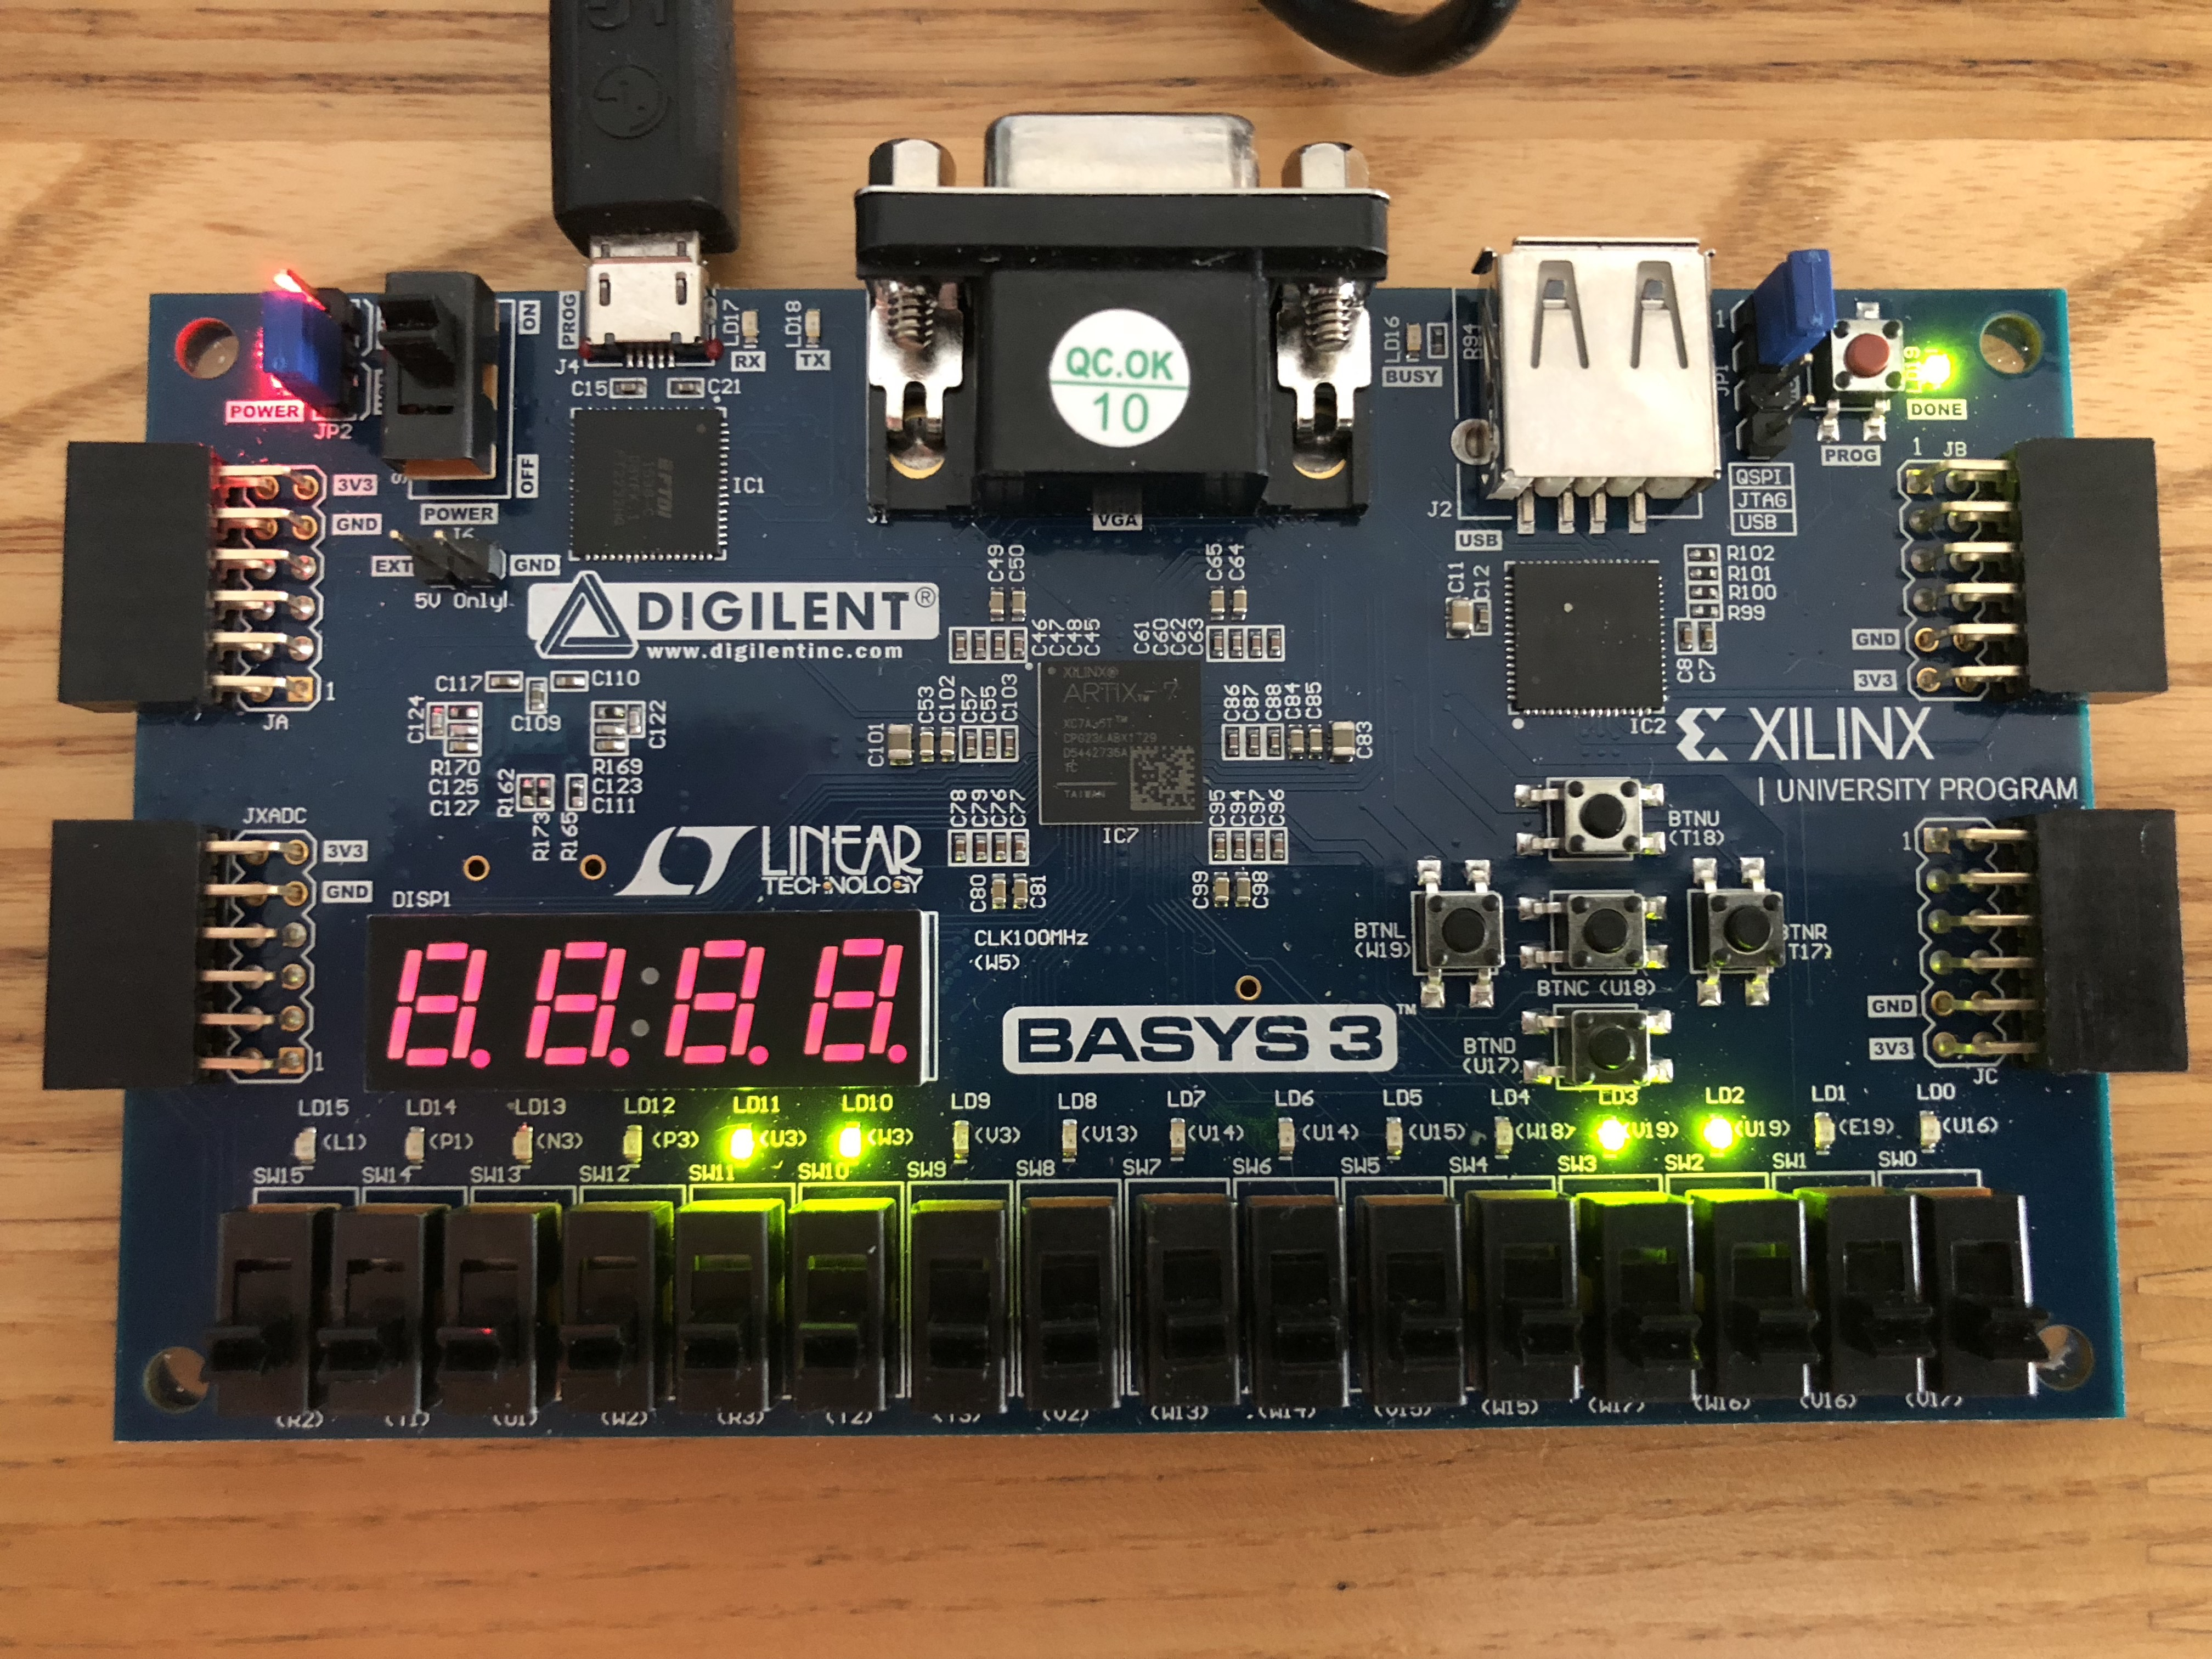
\includegraphics[width=0.5\textwidth]{./images/Part1/l9p1img1.jpg}
	\caption{\label{fig:part1_img1}}
\end{center}
\end{figure}

\begin{figure}[H]
\begin{center}
	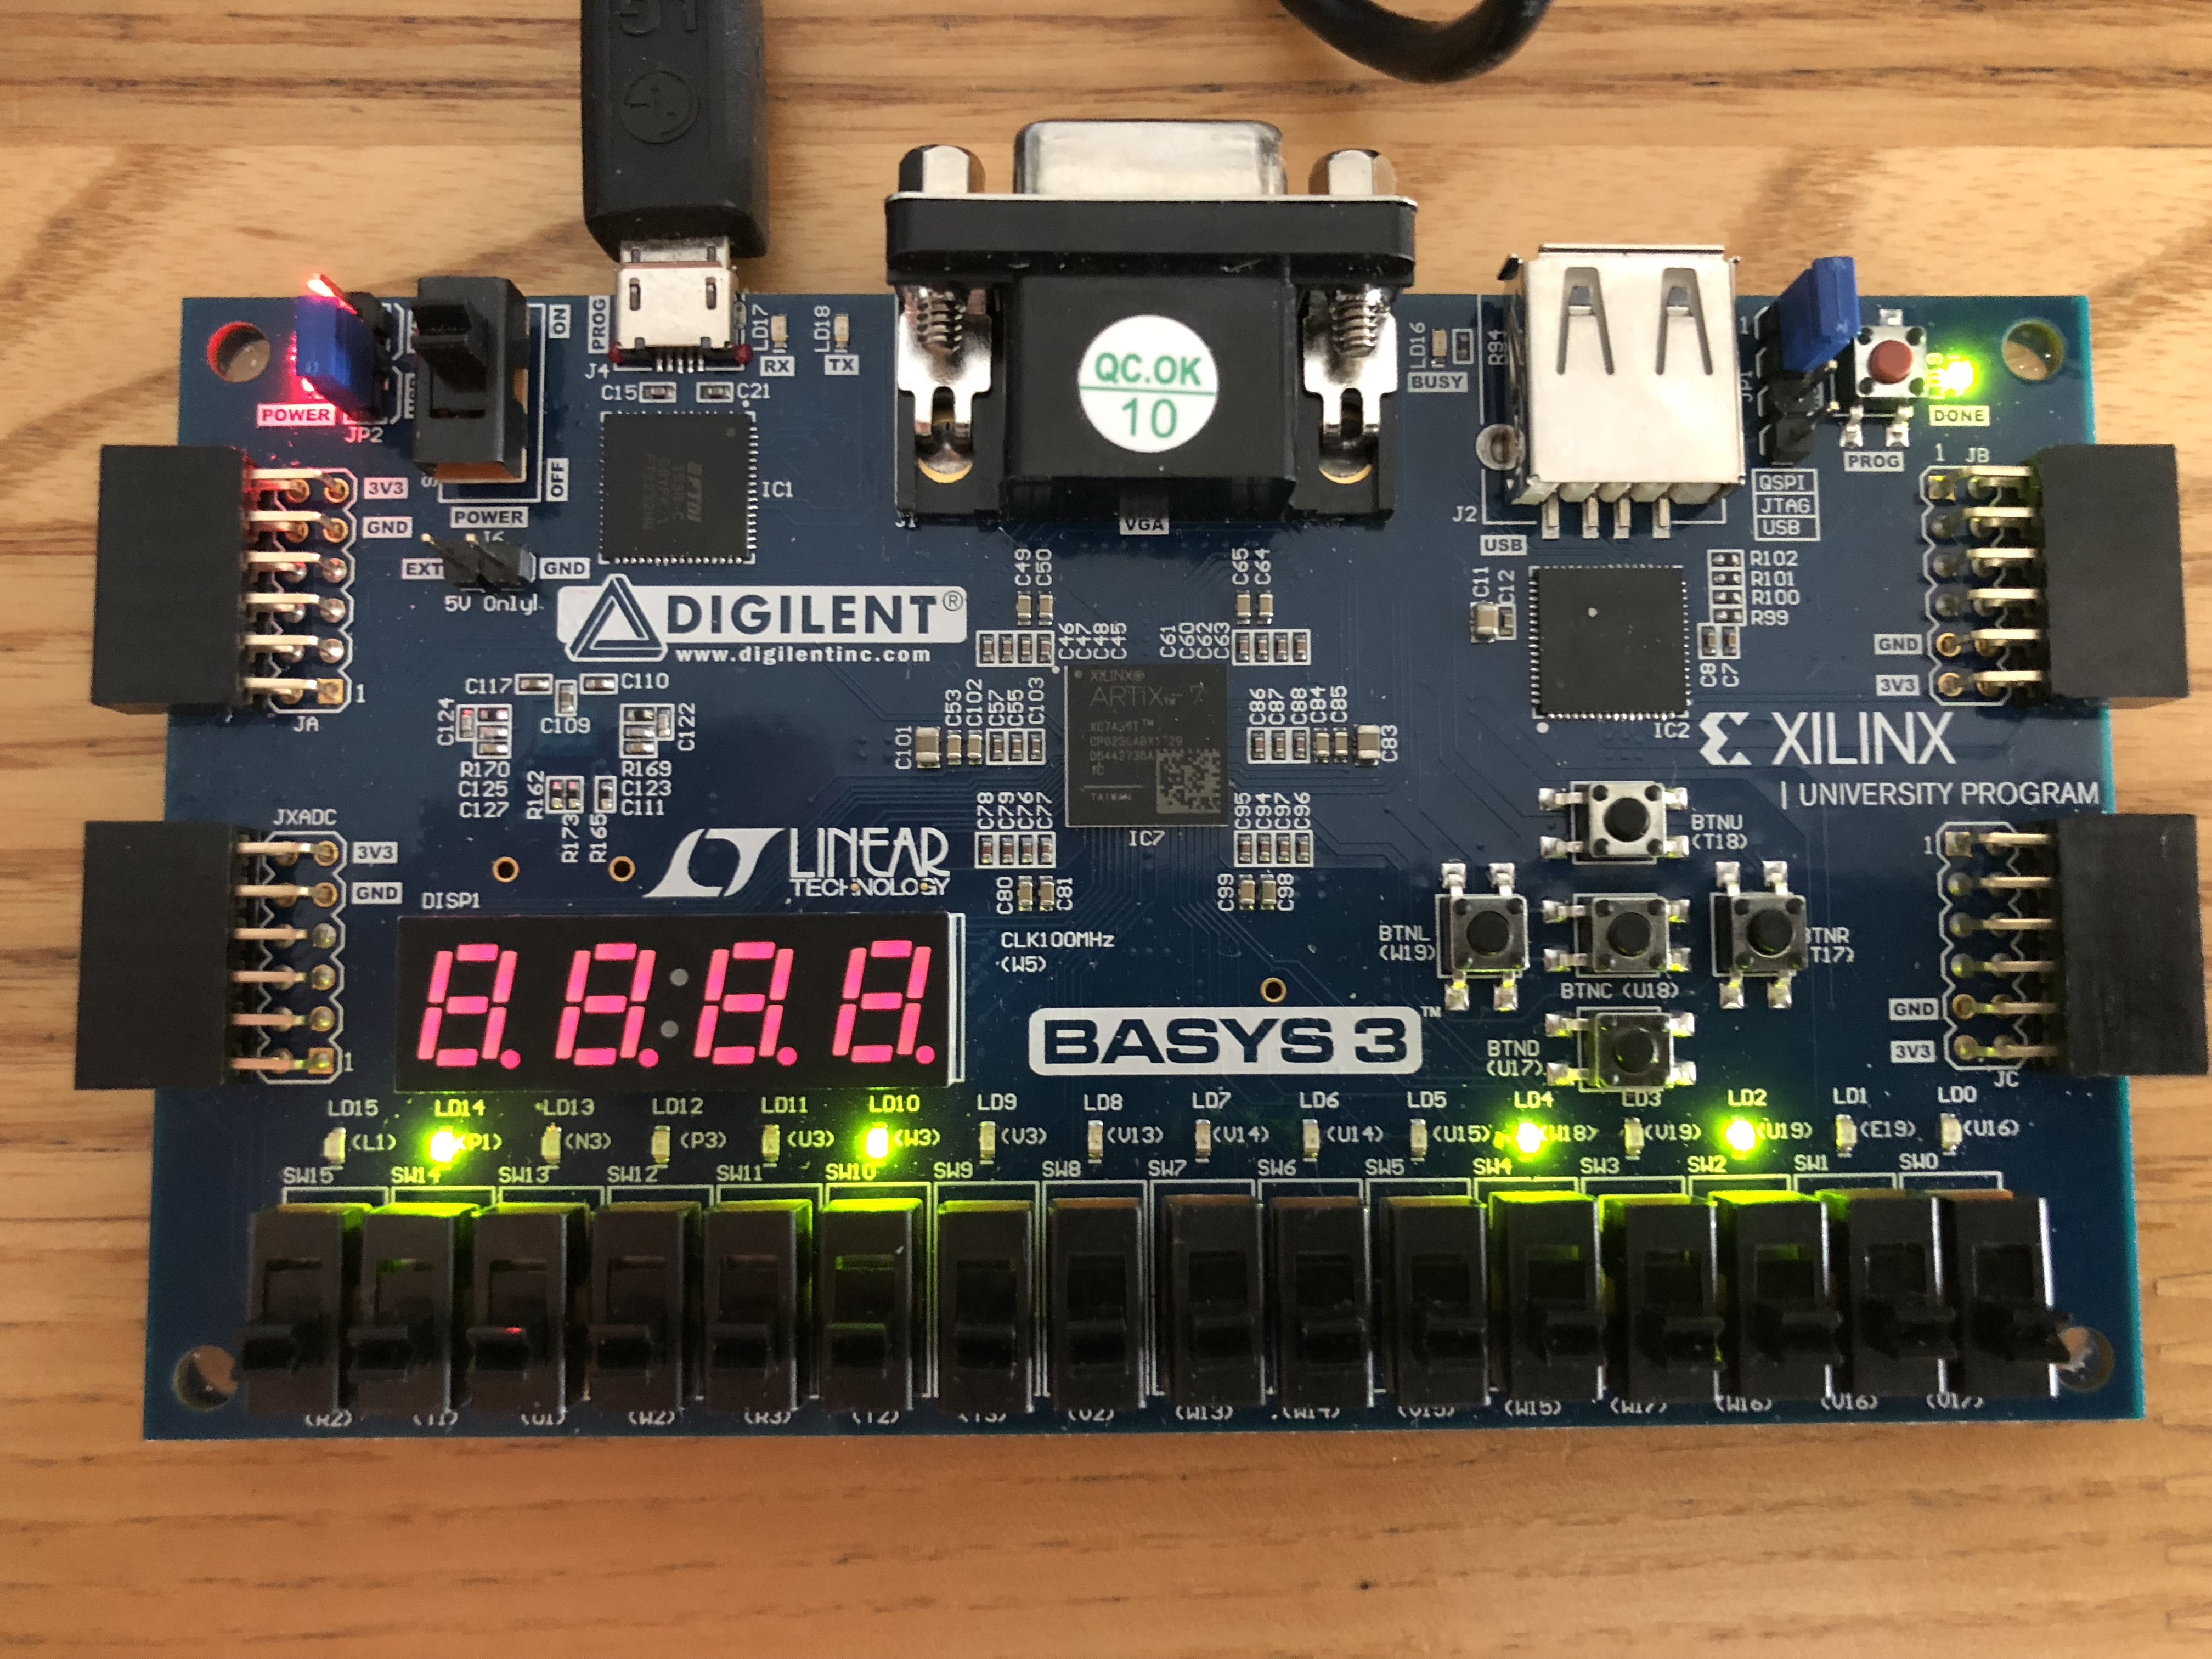
\includegraphics[width=0.5\textwidth]{./images/Part1/l9p1img2.jpg}
	\caption{\label{fig:part1_img2}}
\end{center}
\end{figure}

\begin{figure}[H]
\begin{center}
	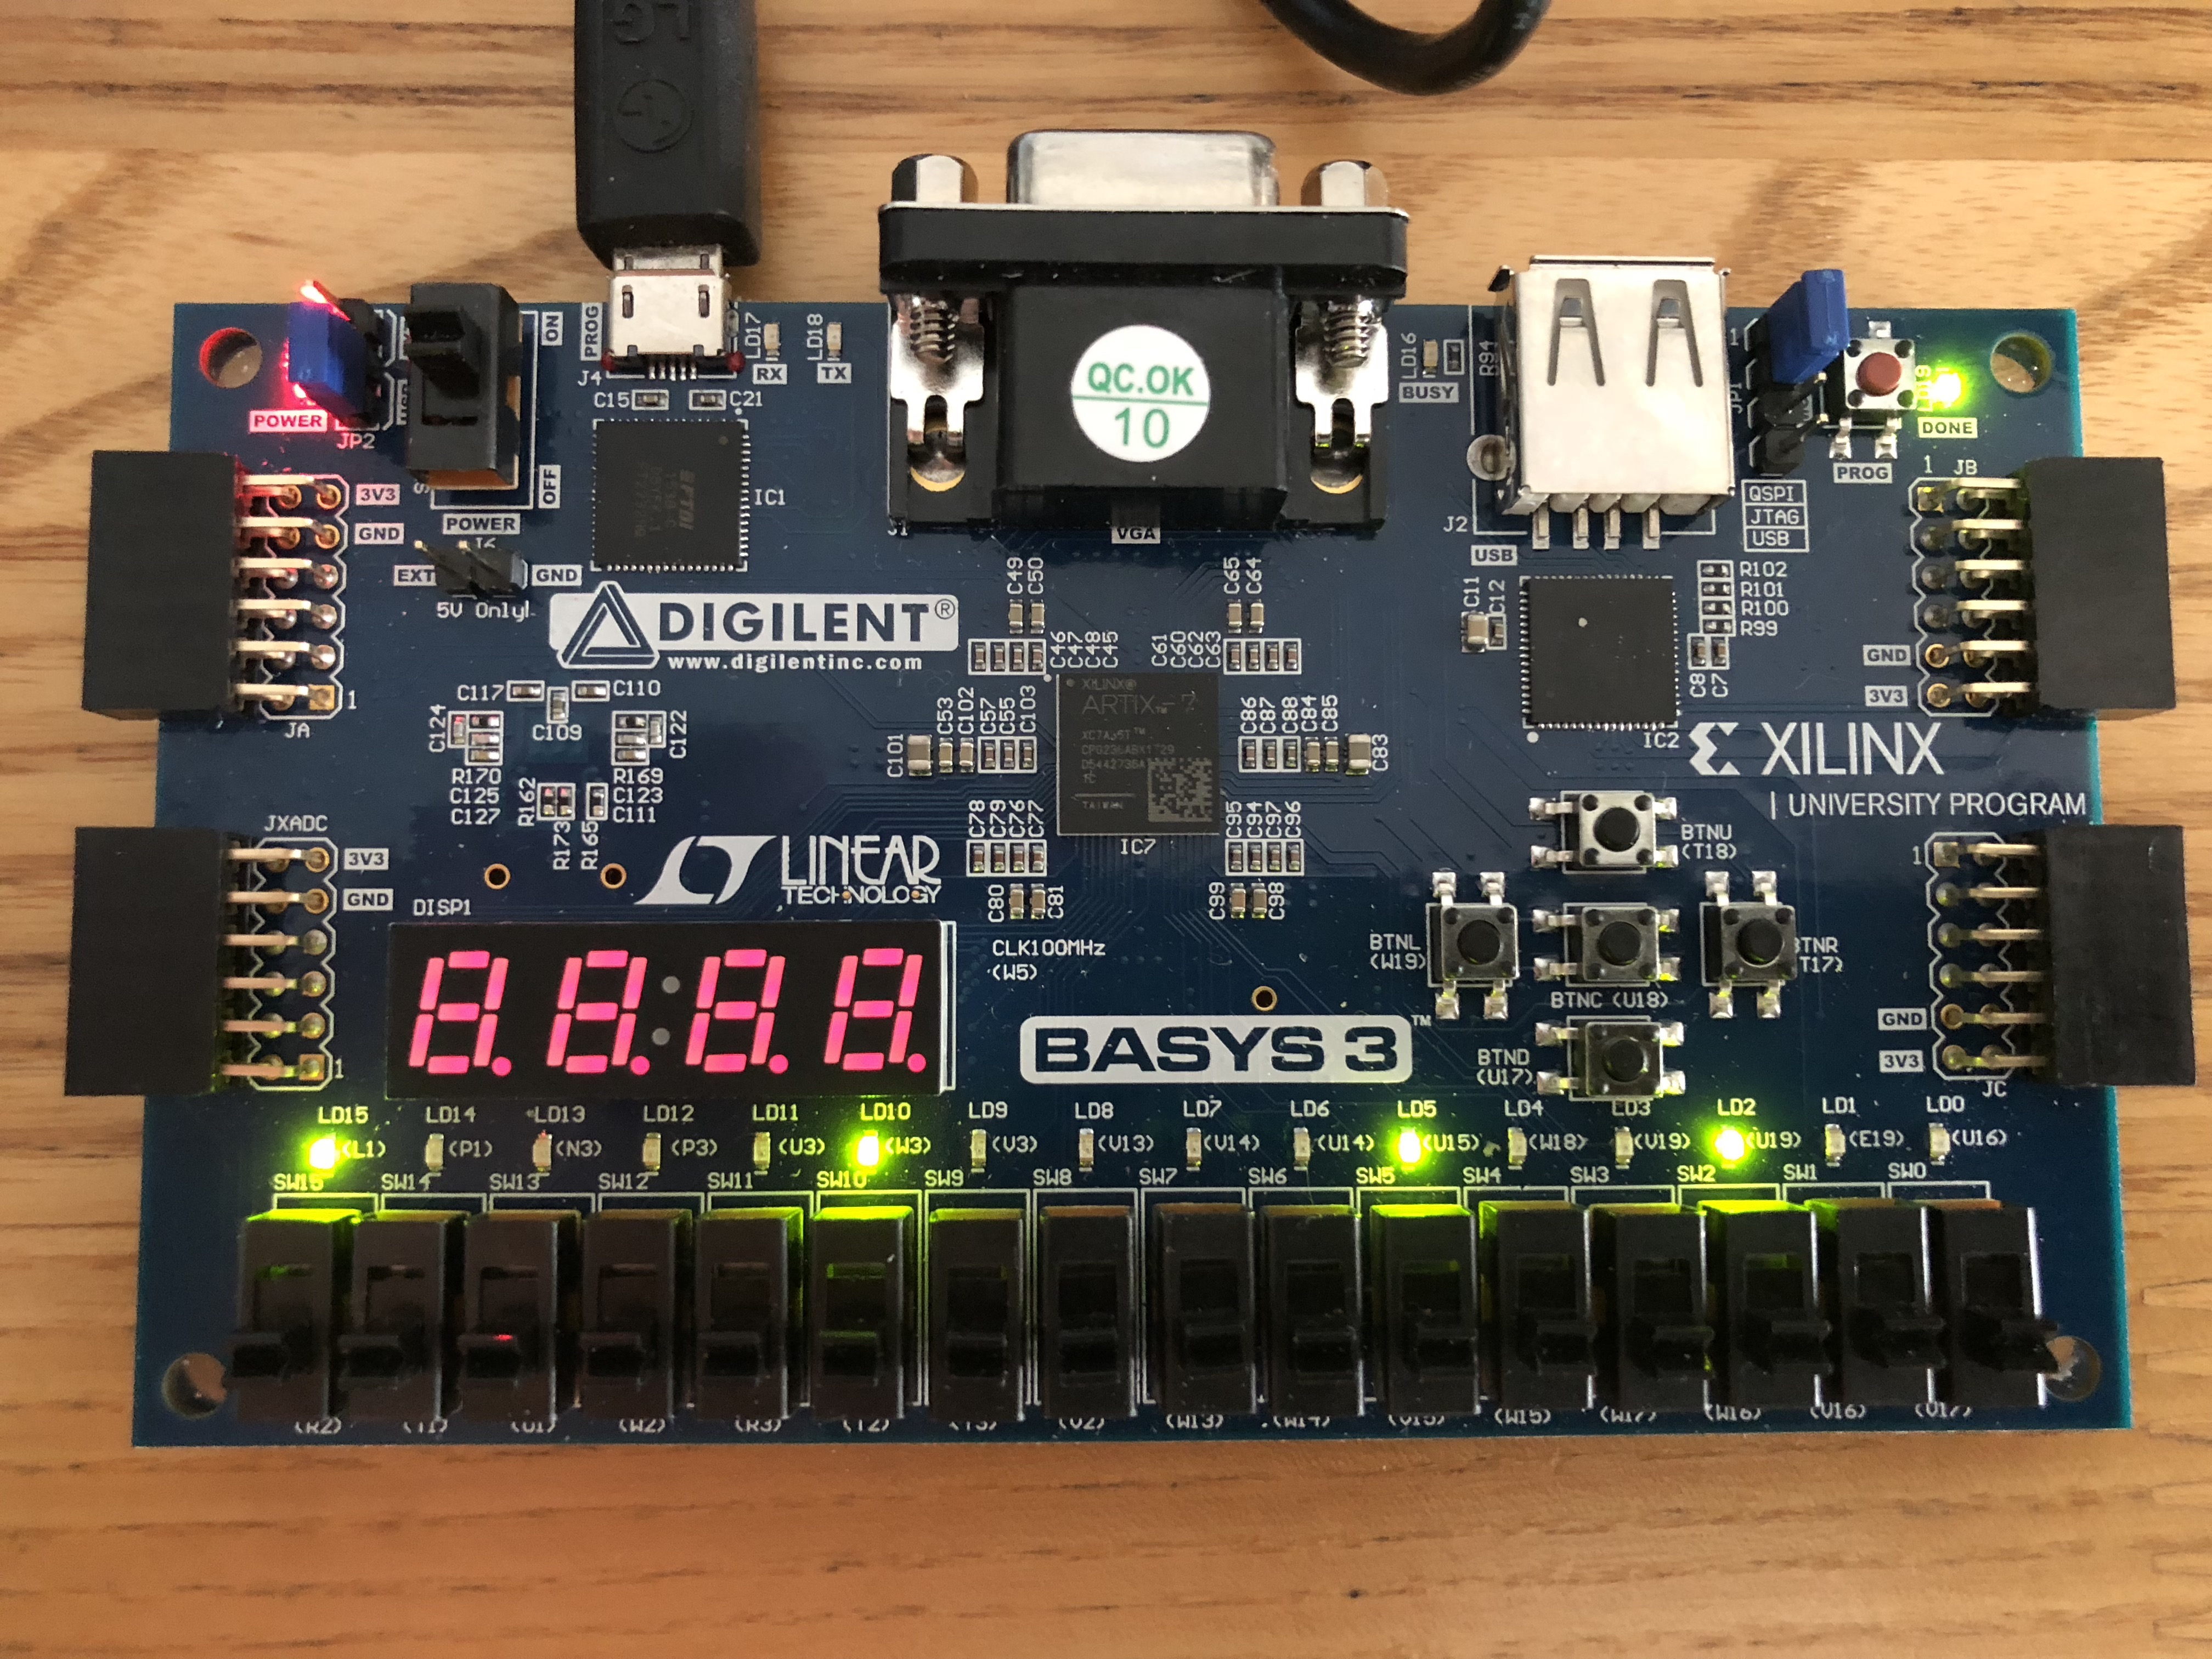
\includegraphics[width=0.5\textwidth]{./images/Part1/l9p1img3.jpg}
	\caption{\label{fig:part1_img3}}
\end{center}
\end{figure}

\begin{figure}[H]
\begin{center}
	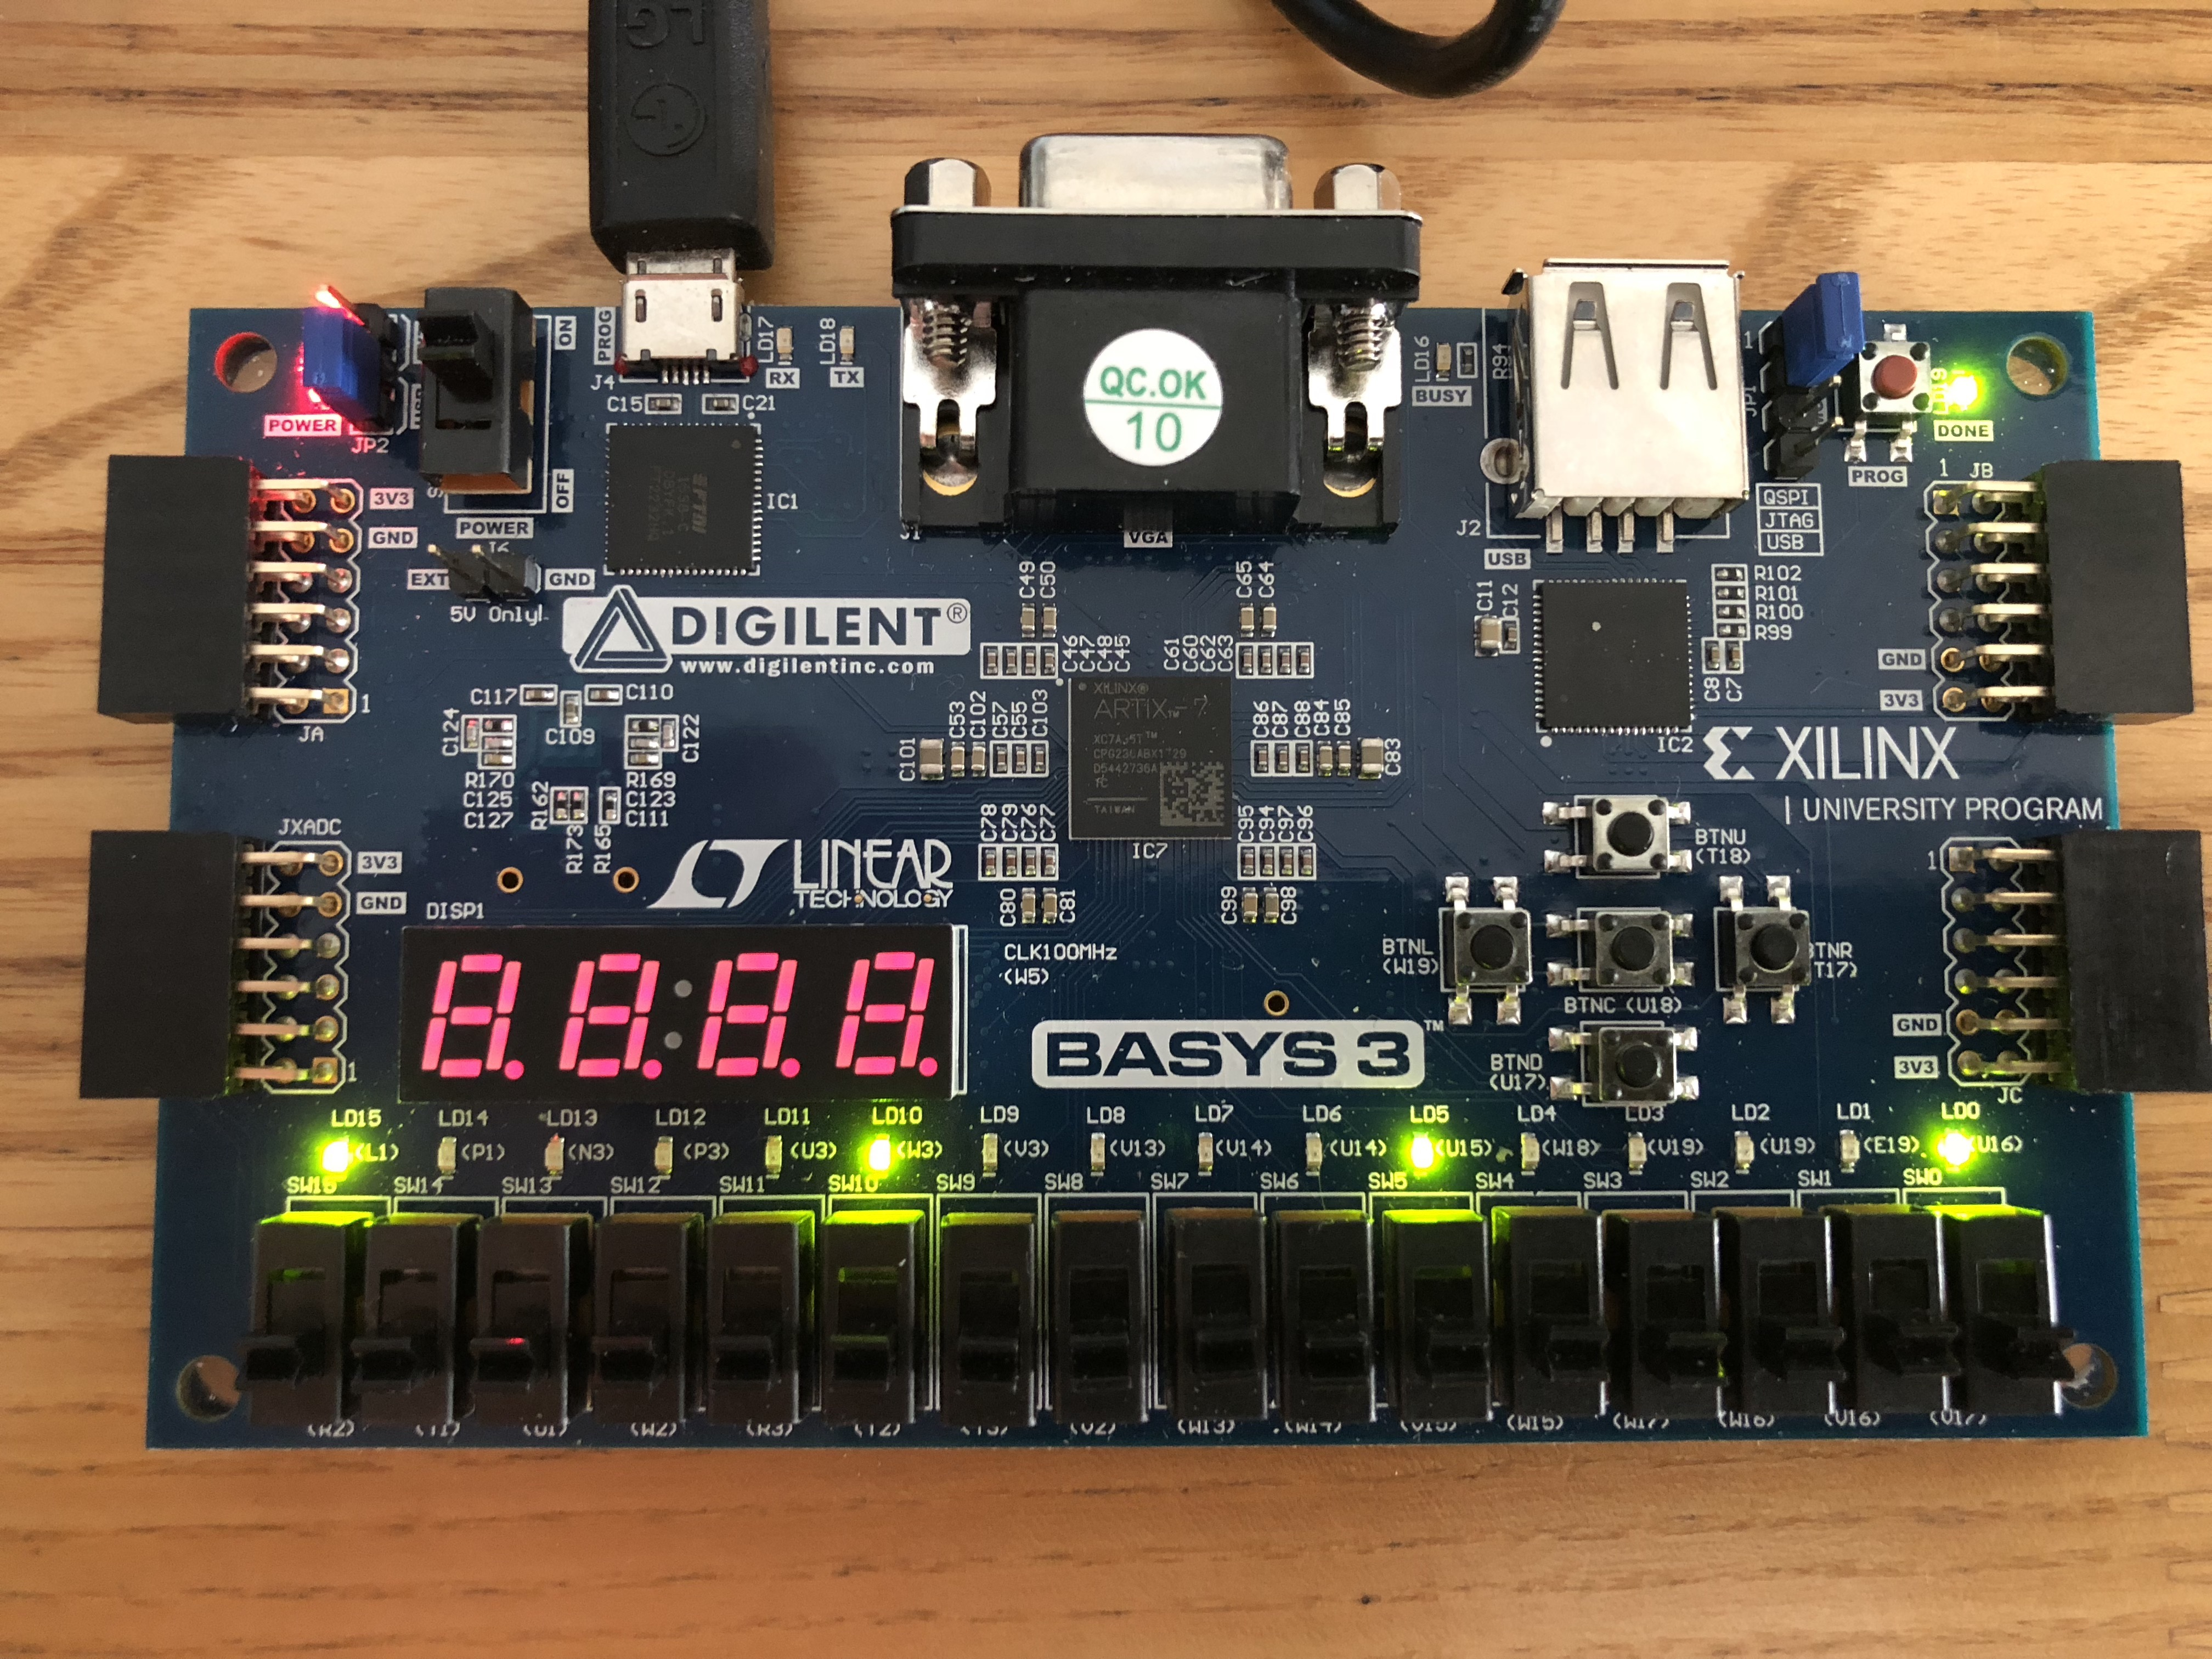
\includegraphics[width=0.5\textwidth]{./images/Part1/l9p1img4.jpg}
	\caption{\label{fig:part1_img4}}
\end{center}
\end{figure}

\begin{figure}[H]
\begin{center}
	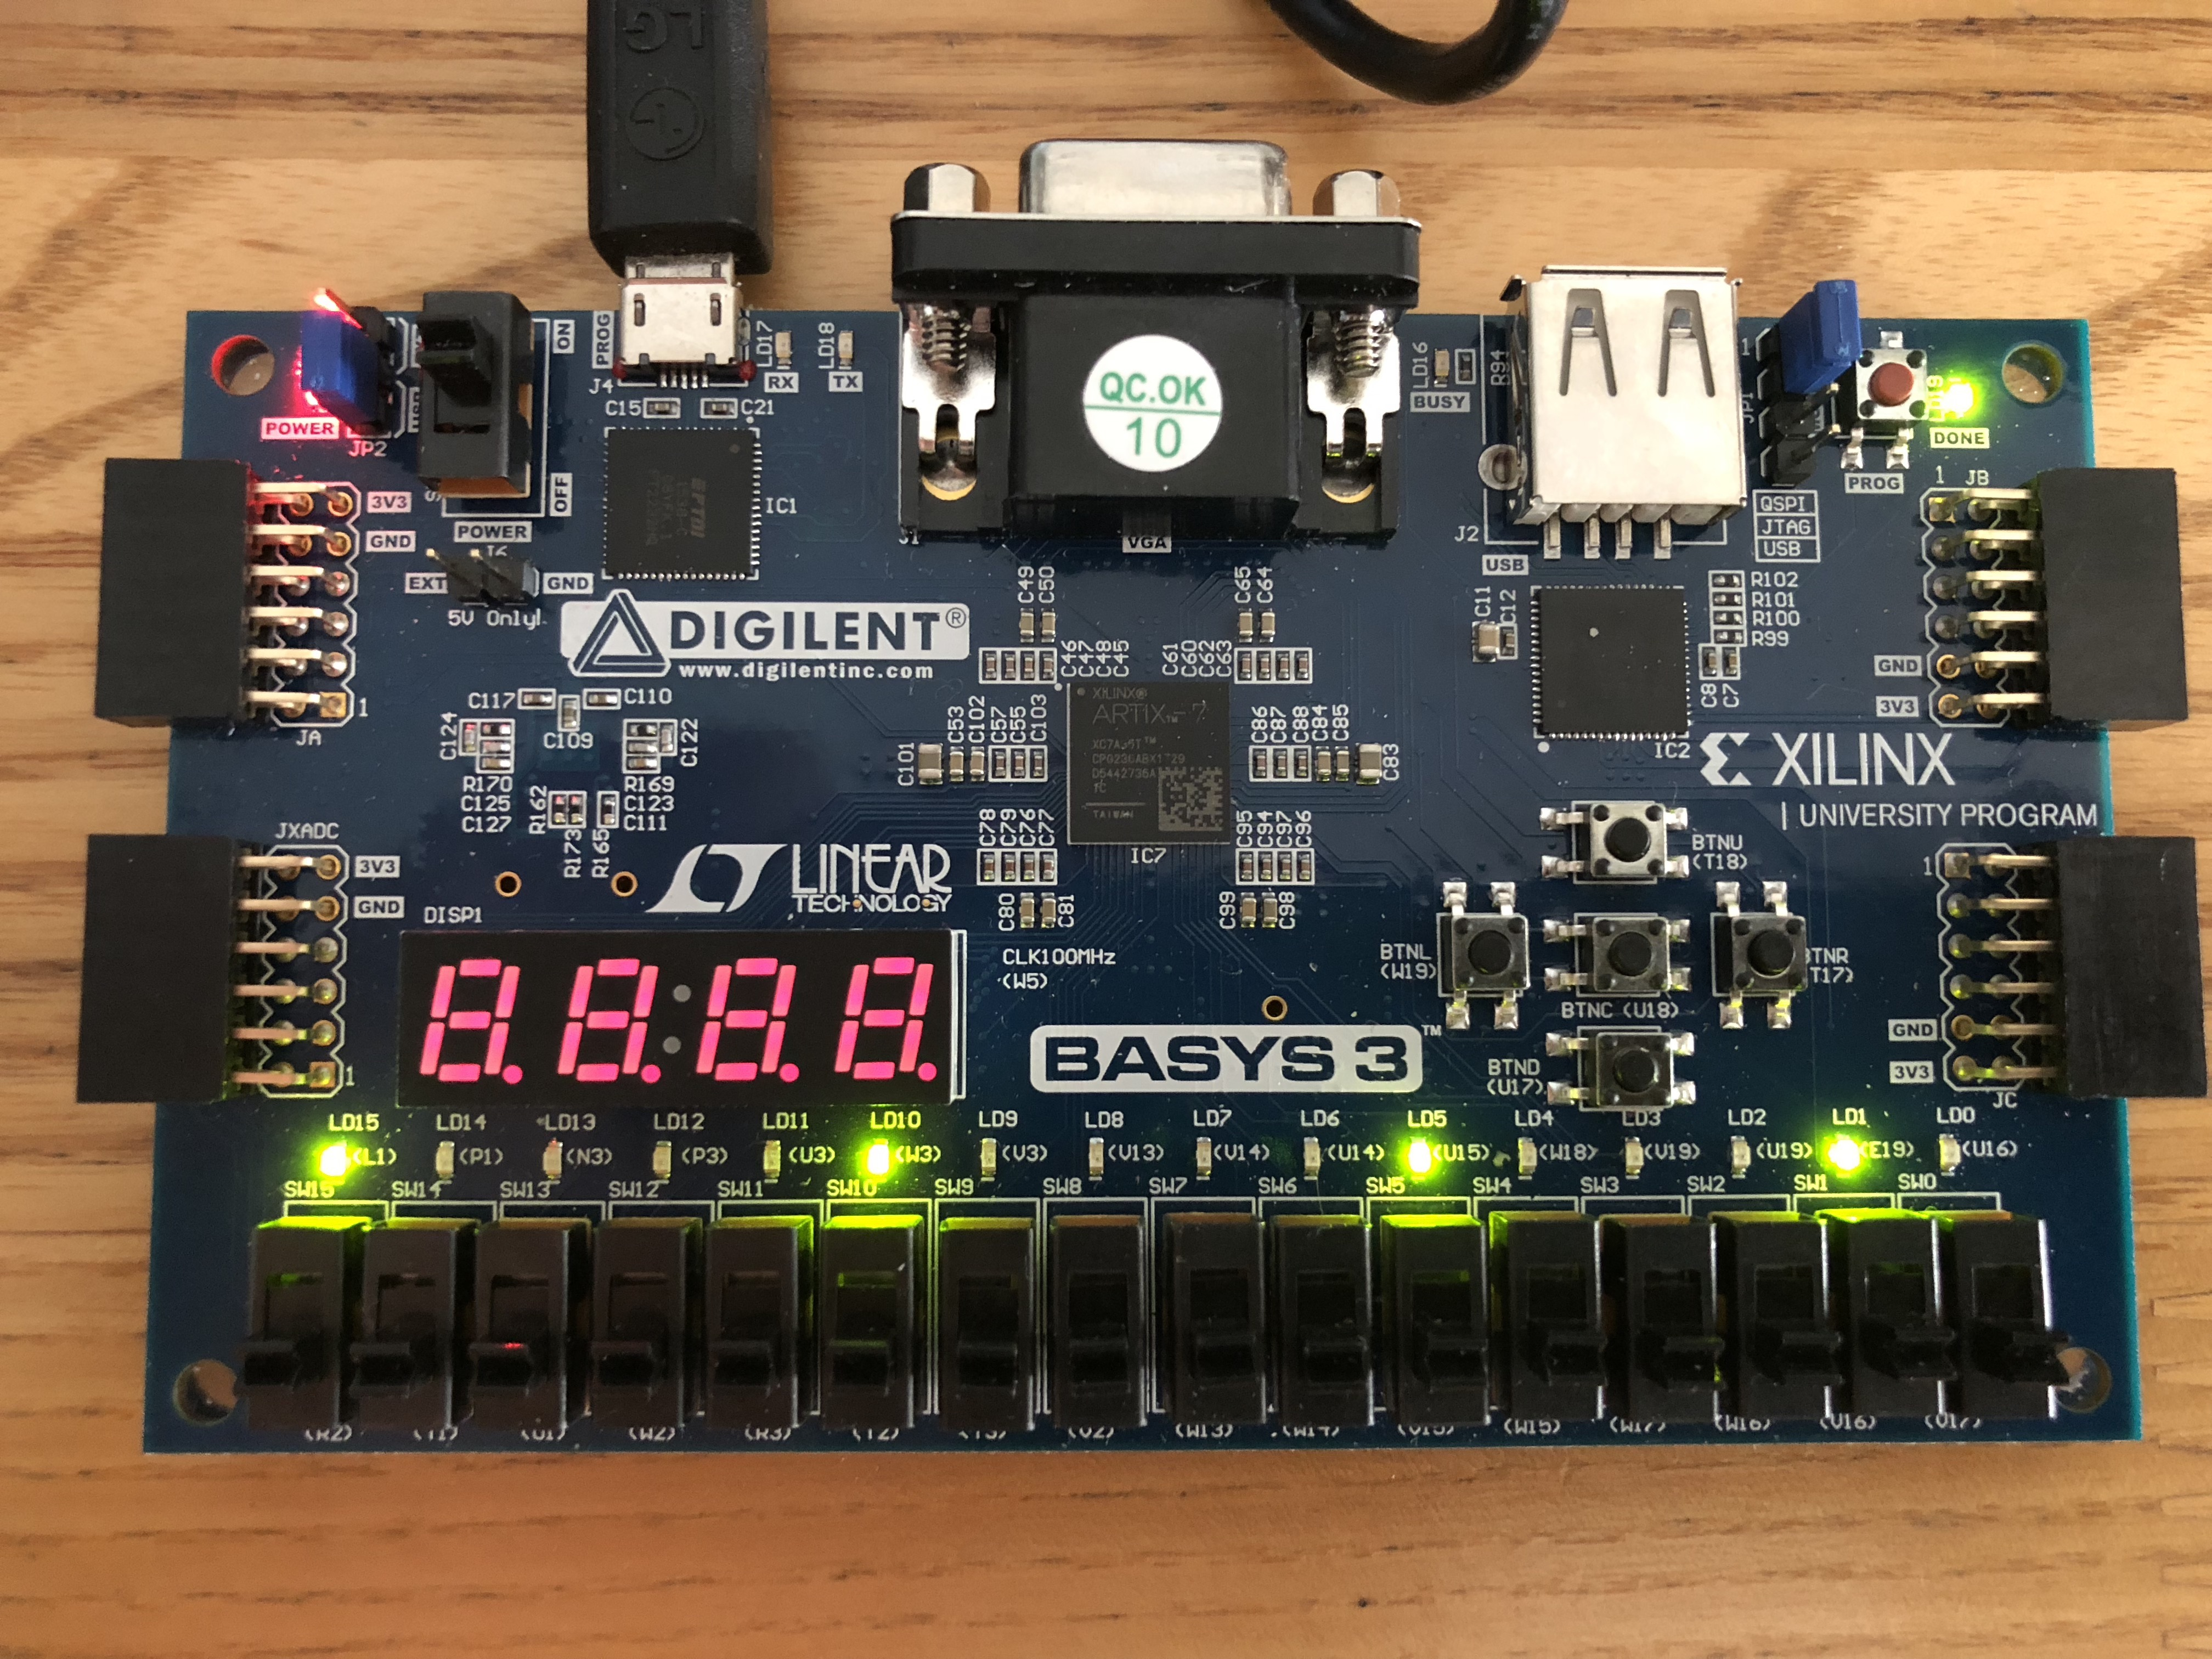
\includegraphics[width=0.5\textwidth]{./images/Part1/l9p1img5.jpg}
	\caption{\label{fig:part1_img5}}
\end{center}
\end{figure}

\begin{figure}[H]
\begin{center}
	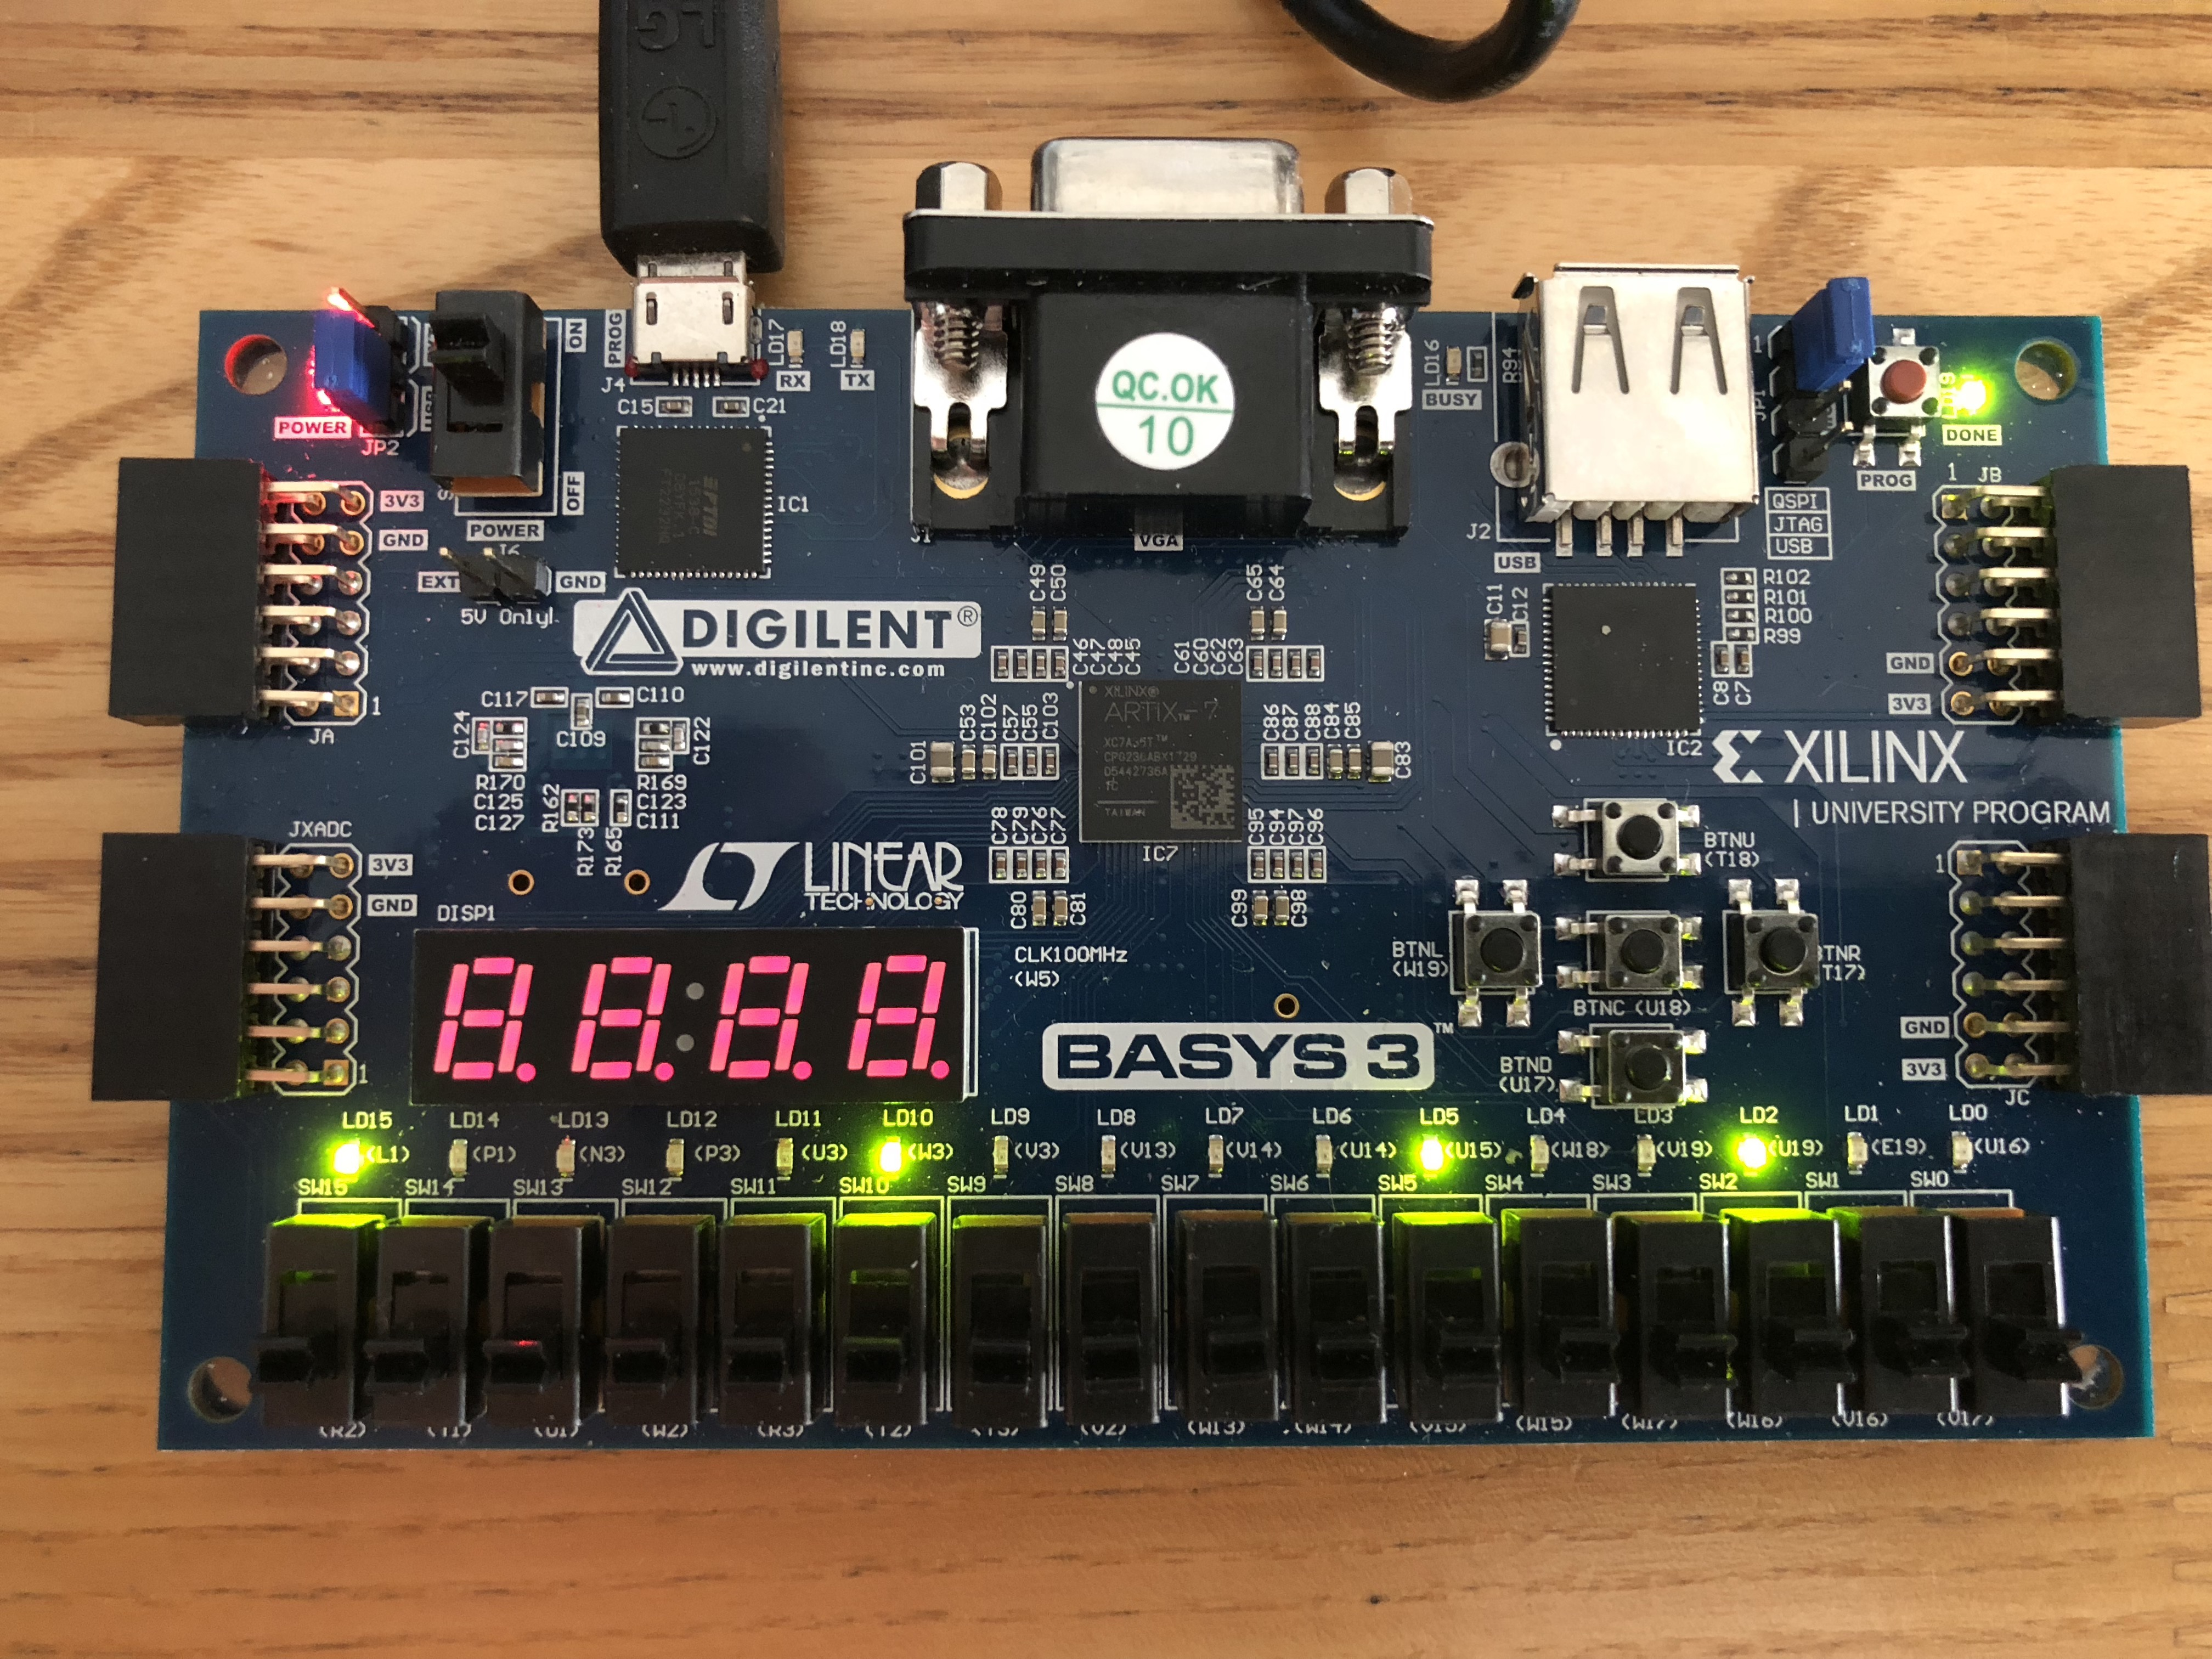
\includegraphics[width=0.5\textwidth]{./images/Part1/l9p1img6.jpg}
	\caption{\label{fig:part1_img6}}
\end{center}
\end{figure}

\begin{figure}[H]
\begin{center}
	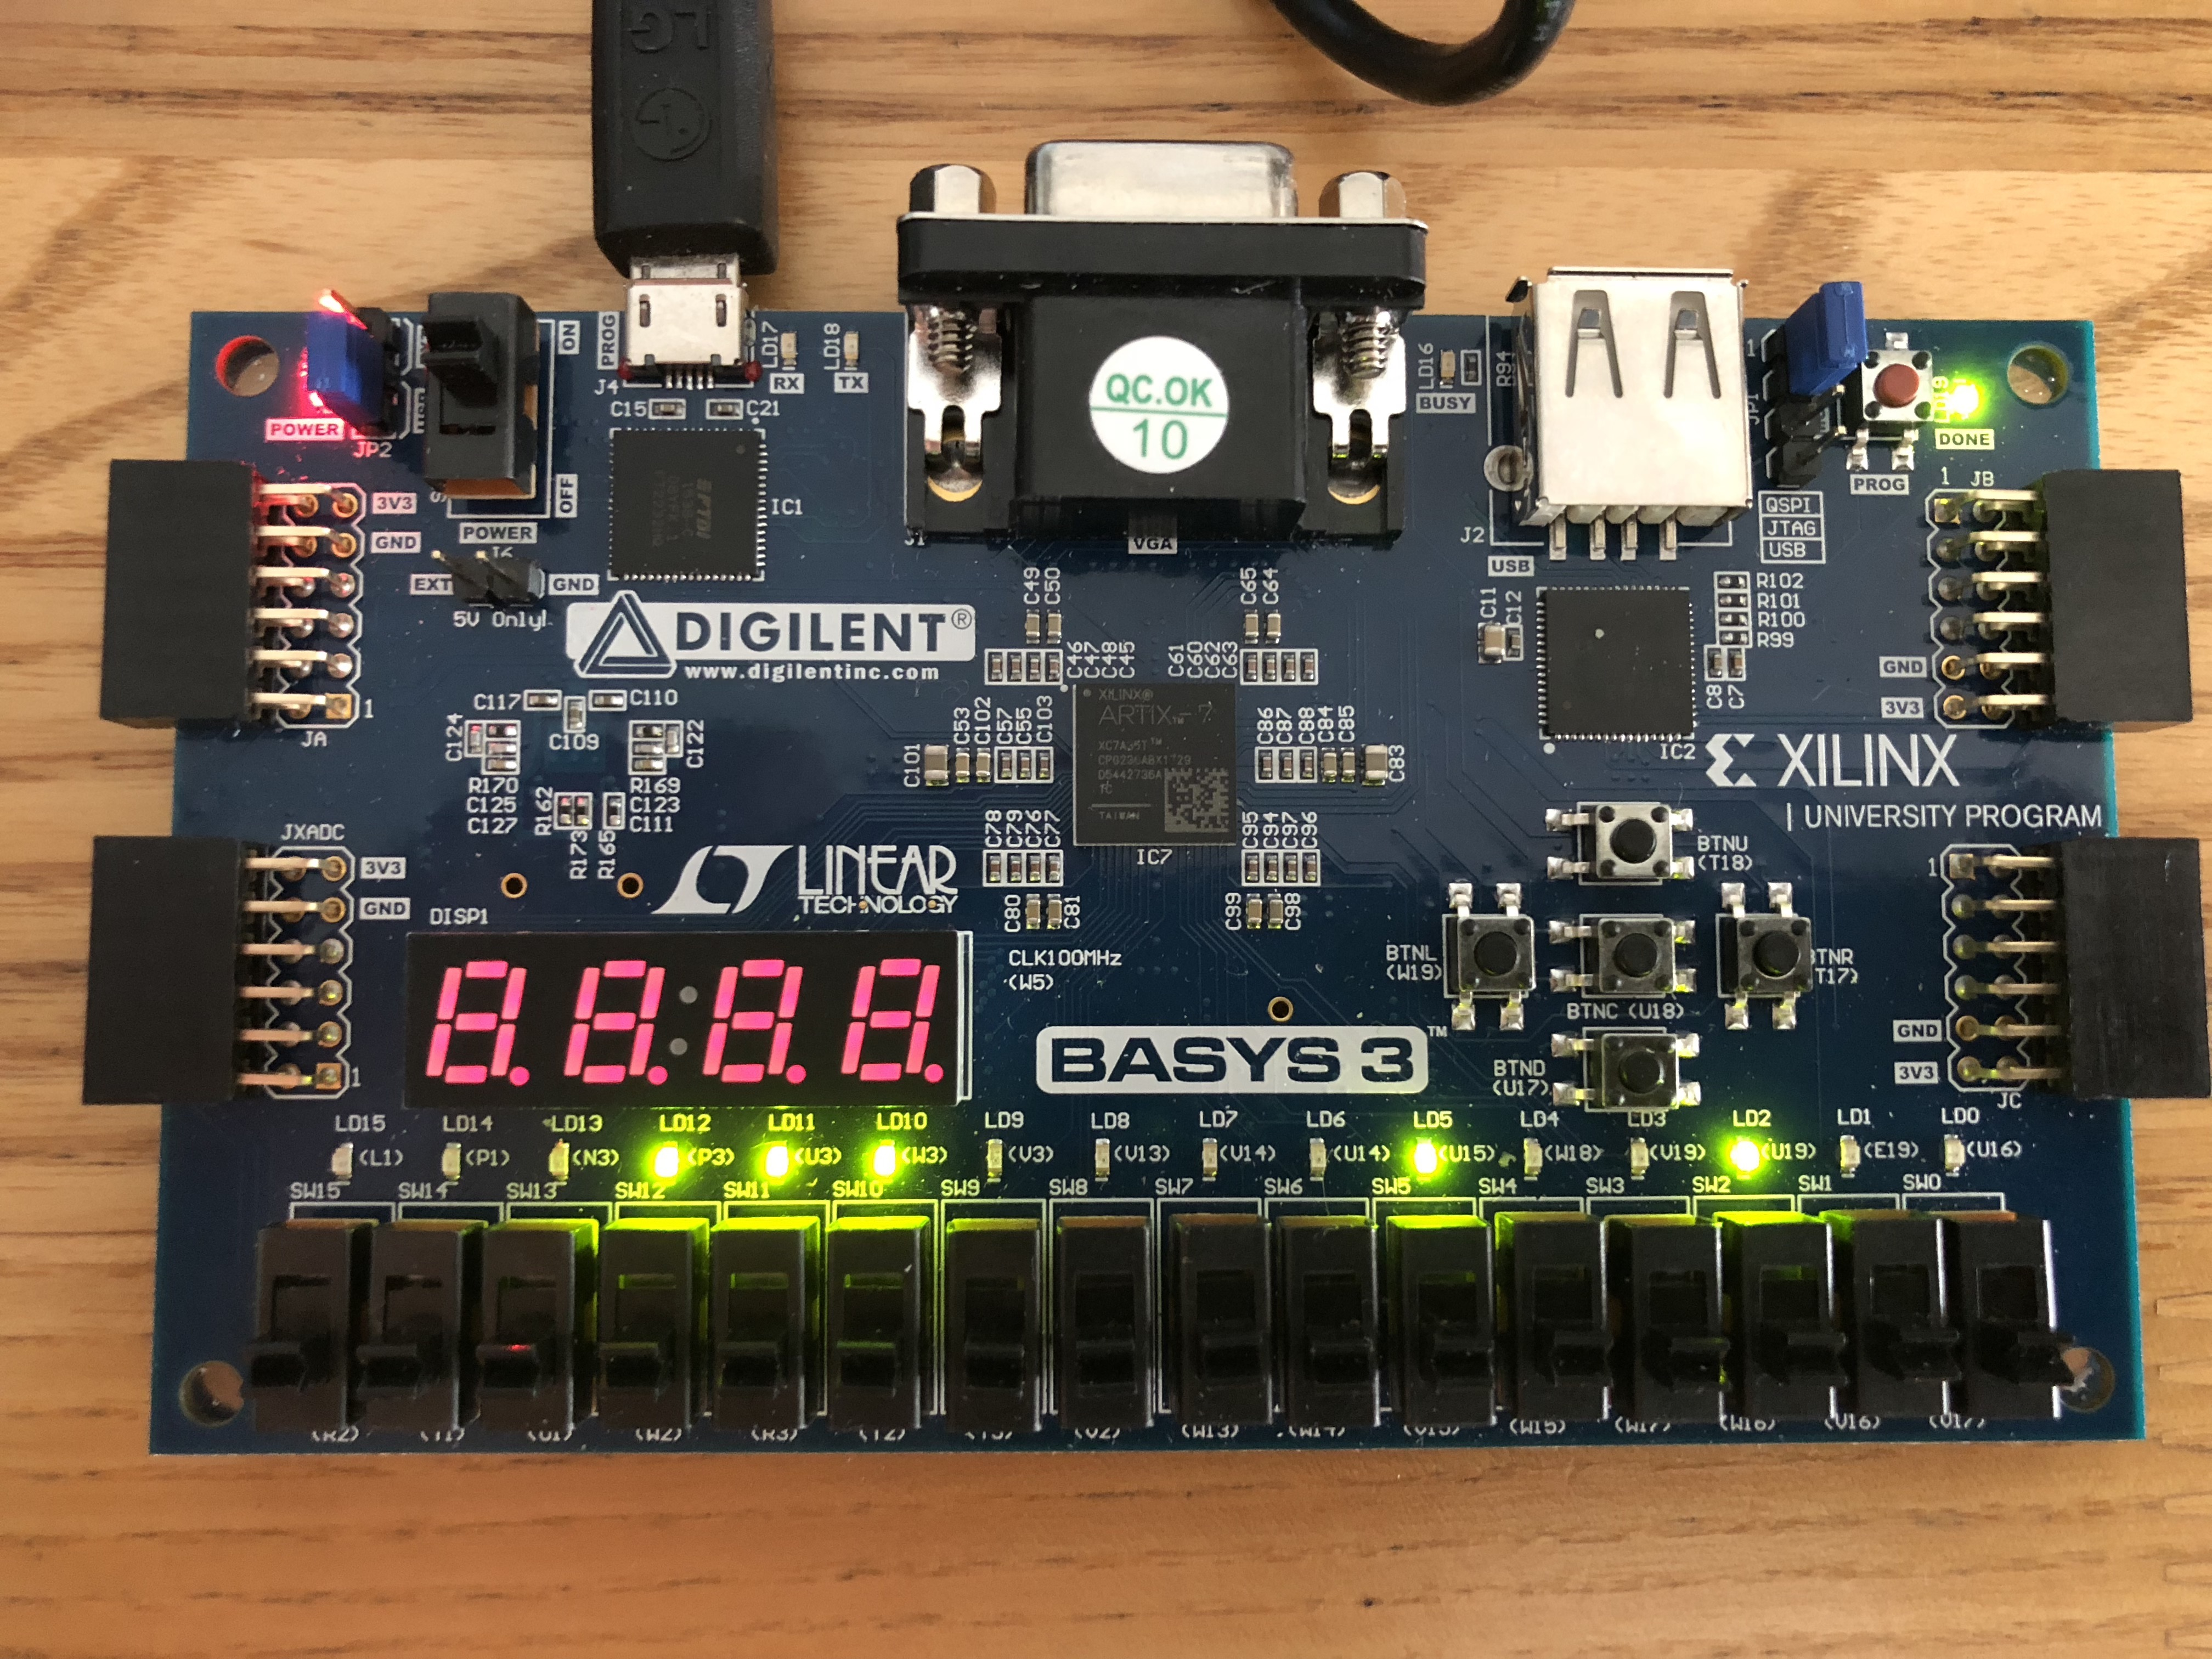
\includegraphics[width=0.5\textwidth]{./images/Part1/l9p1img7.jpg}
	\caption{\label{fig:part1_img7}}
\end{center}
\end{figure}

\begin{figure}[H]
\begin{center}
	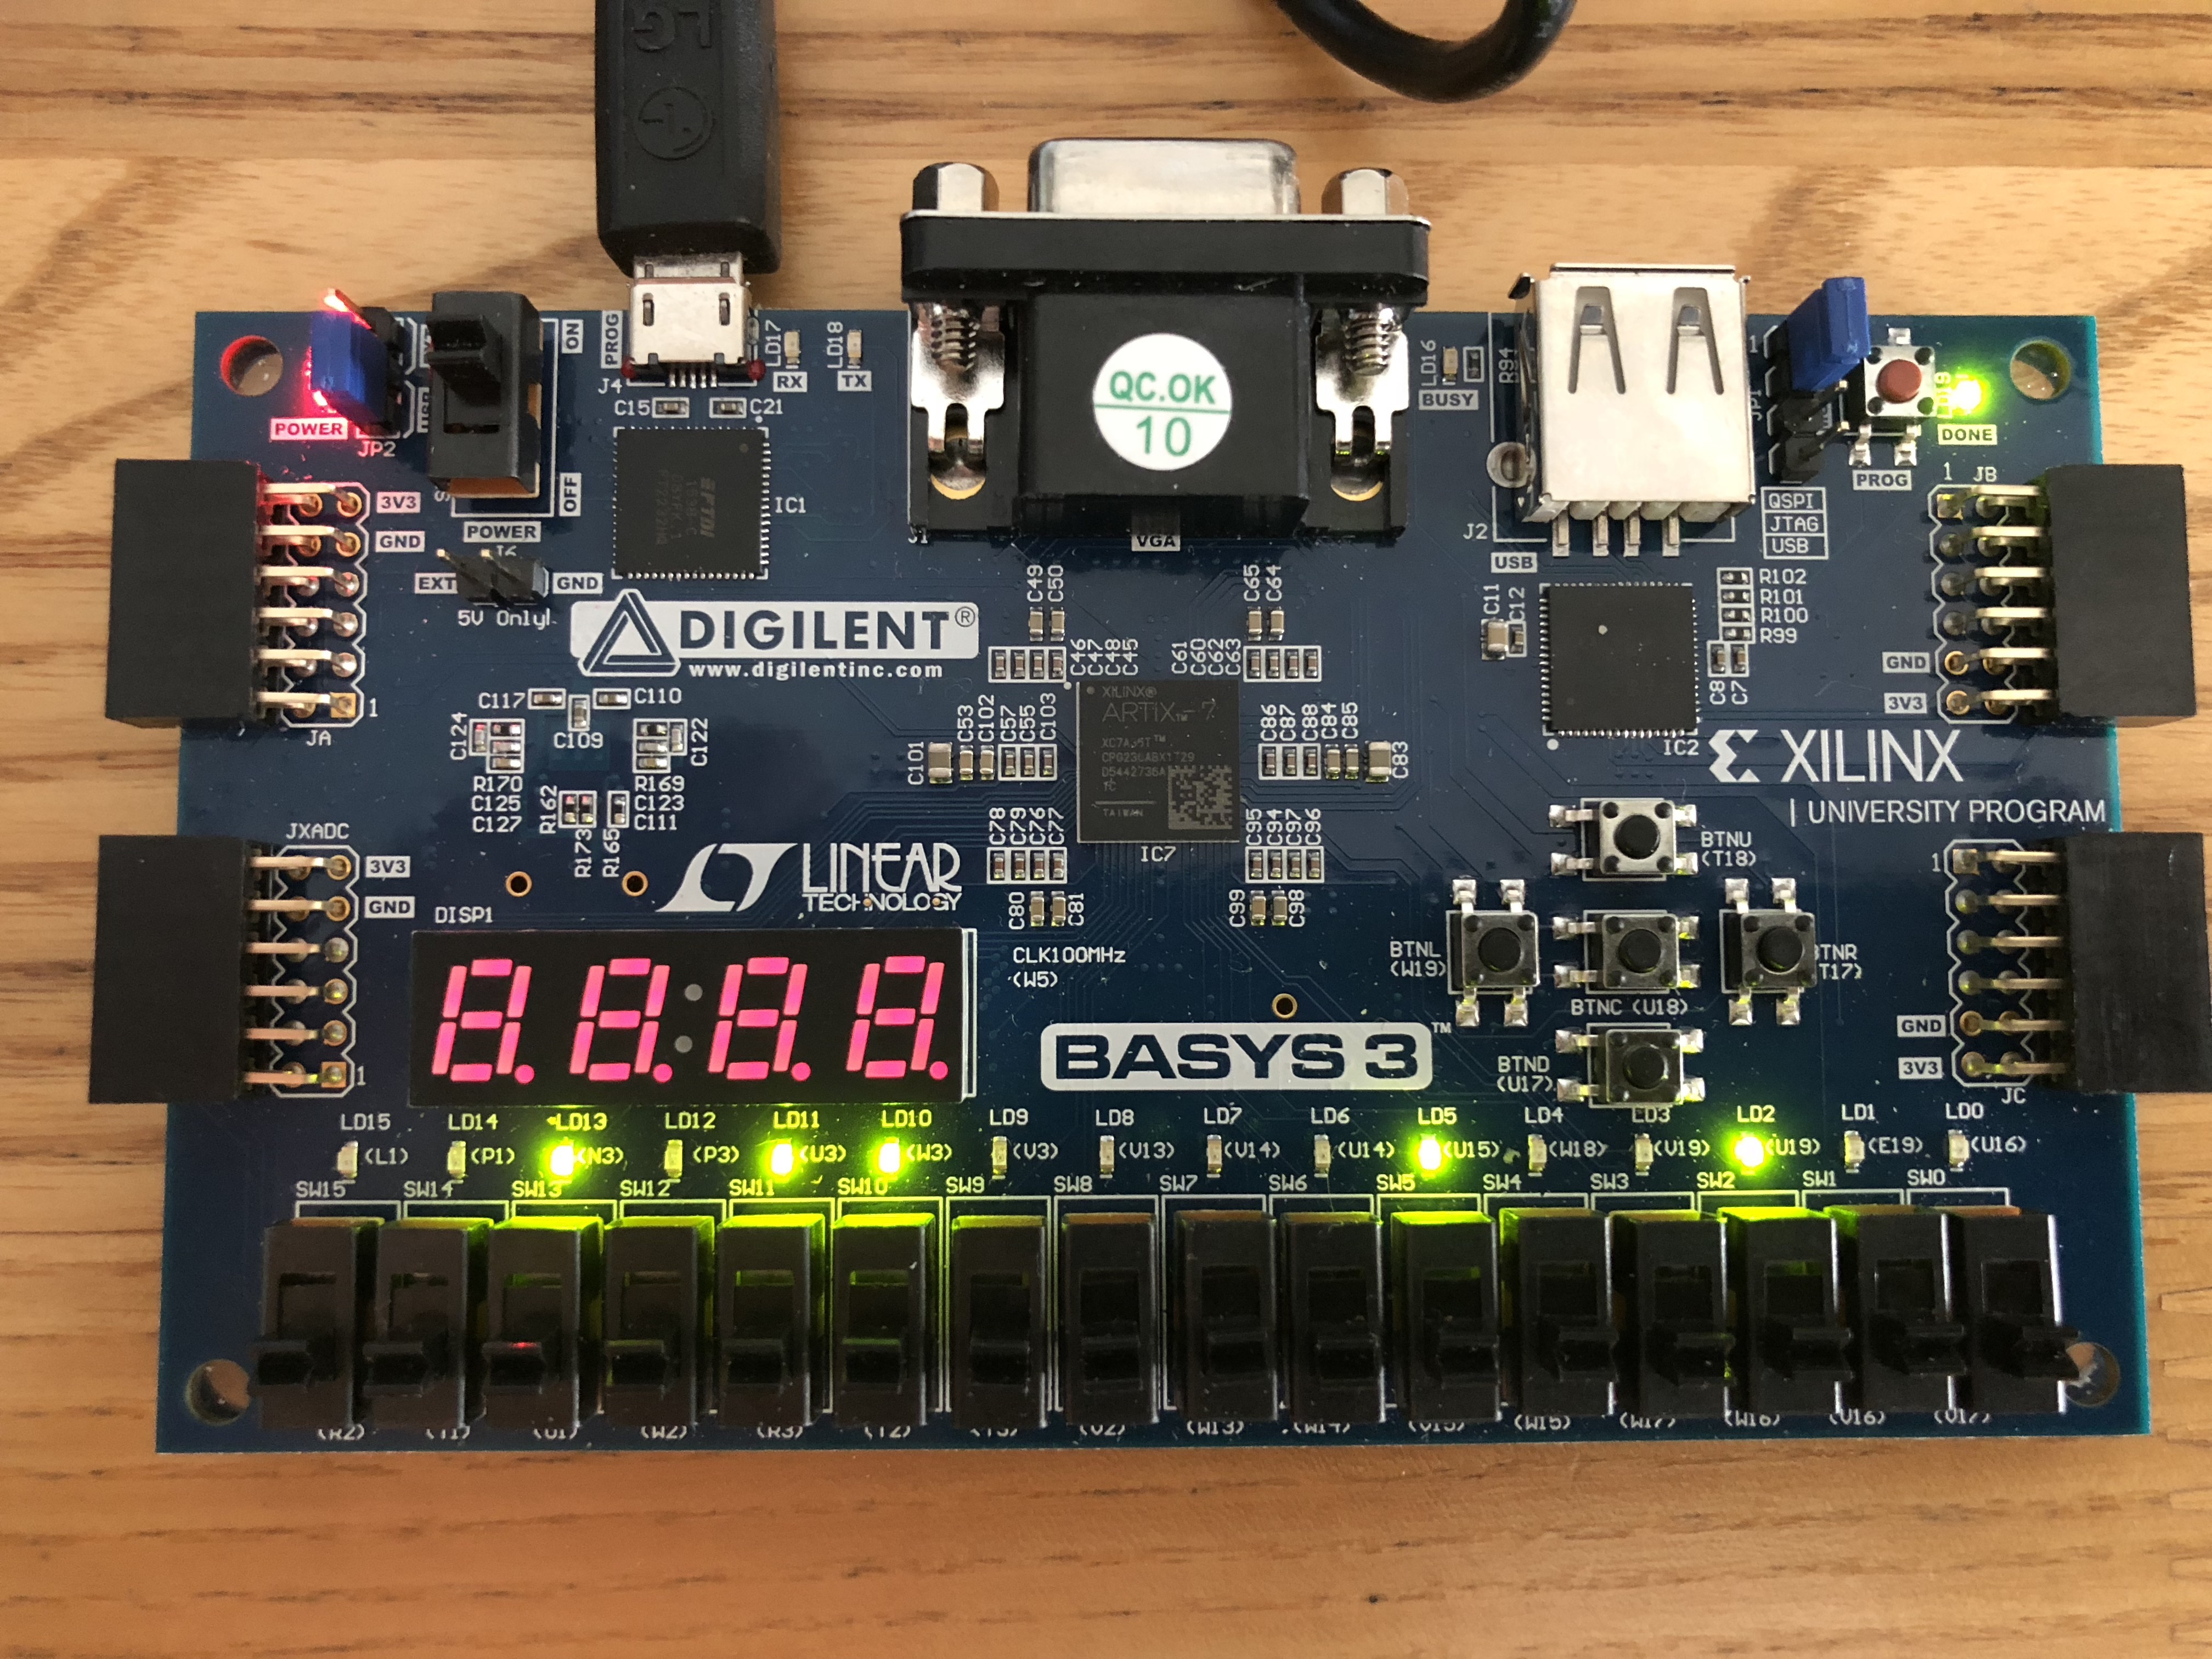
\includegraphics[width=0.5\textwidth]{./images/Part1/l9p1img8.jpg}
	\caption{\label{fig:part1_img8}}
\end{center}
\end{figure}

\begin{figure}[H]
\begin{center}
	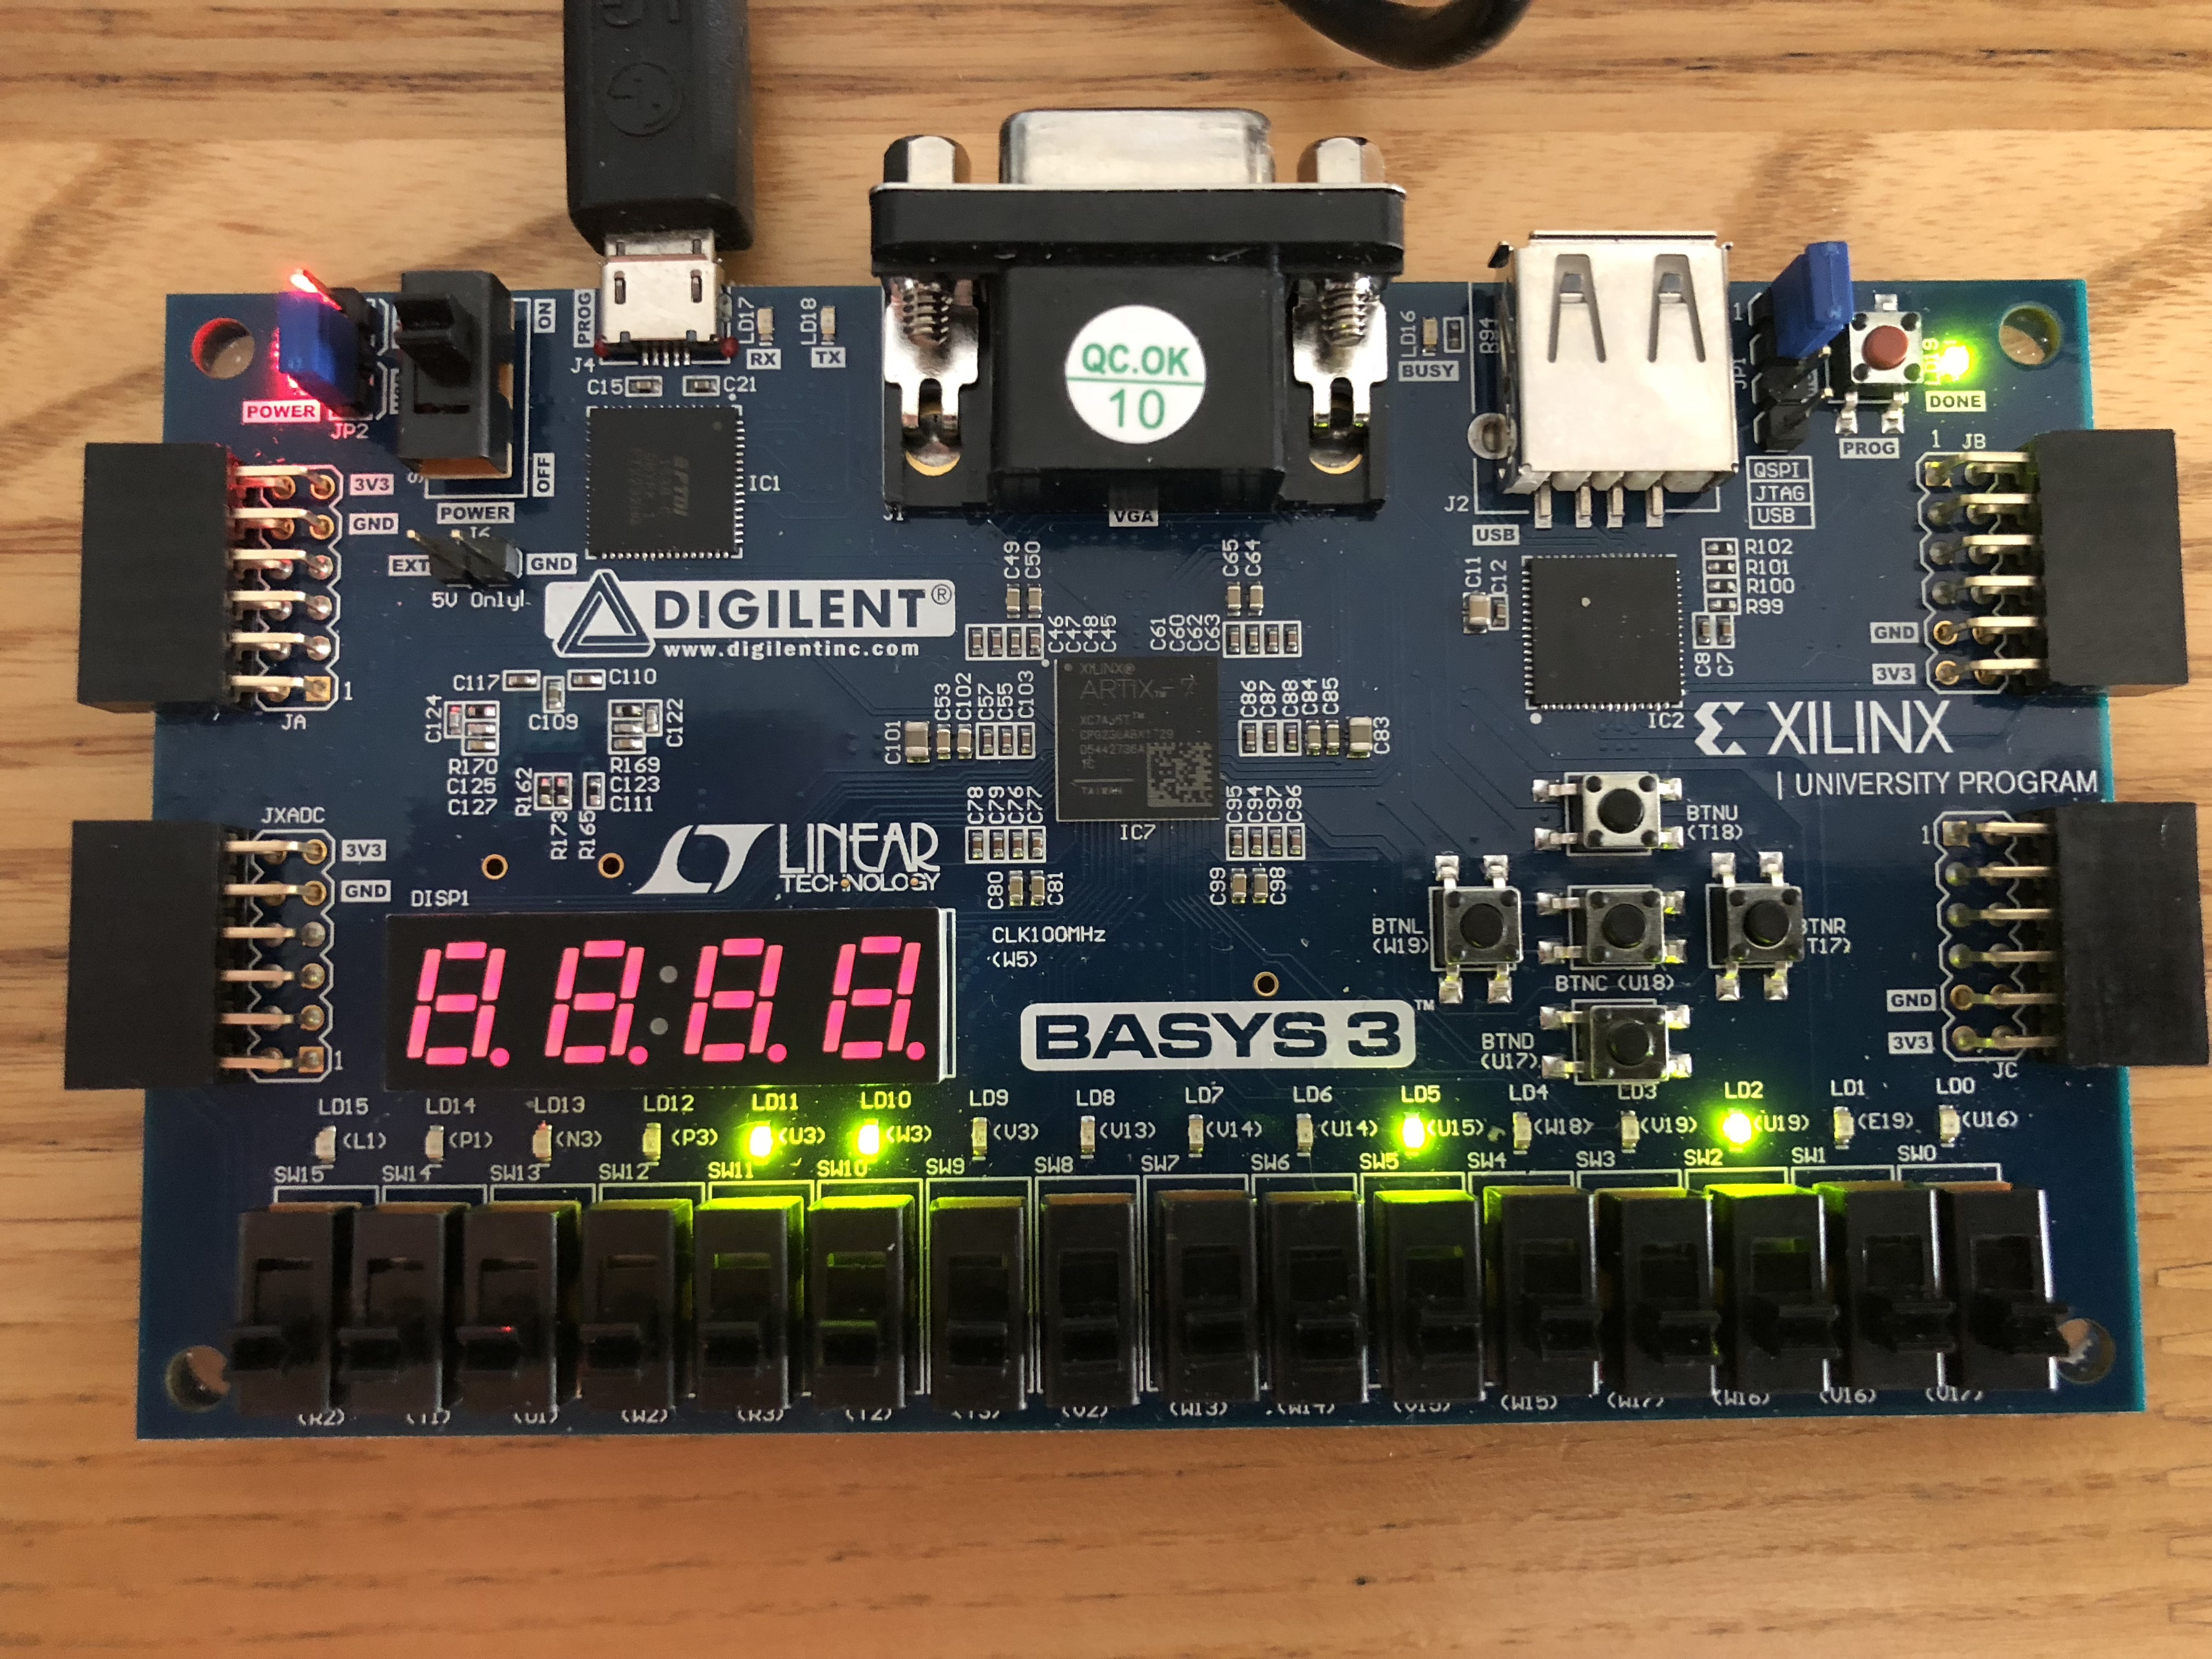
\includegraphics[width=0.5\textwidth]{./images/Part1/l9p1img9.jpg}
	\caption{\label{fig:part1_img9}}
\end{center}
\end{figure}


\subsection{Problem 2 }

\subsubsection{Background}
For Problem 2, we are required to add wrap-around functionality, load, enable, and synchronous reset to the counter from Problem 1.

\subsubsection{Design Solution}
Some functionality, such as reset and enable, already existed from the previous problem, where we found it easier to implement a synchronous design with these things than without them. For this problem, they just had to be given input ports. The input ports are summarized in Table ~\ref{tab:advanced_counter_input_Ports} and the output ports are summarized in ~\ref{tab:advanced_counter_output_Ports}. For the load operation, we decided to accept a 4-bit number so that we could inititalize the counter to any value that it could normally count to, 0 through 9. Any value greater than 9 ("1001") automatically results in the counter being set to 0.

\begin{table}[H]
\begin{center}
\begin{tabular}{| l | l | l |}
	\hline
	Bit & Label & Port \\ \hline
	clk &  Clock & W5 \\ \hline
	direction & Switch 0 & V17 \\ \hline
	load & Switch 1 & V16 \\ \hline
	enable & Switch 2 & W16 \\ \hline
	reset & Button Right & T17 \\ \hline
	input3 & Switch 15 & R2 \\ \hline
	input2 & Switch 14 & T1 \\ \hline
	input1 & Switch 13 & U1 \\ \hline
	input 0 & Switch 12 & W2 \\ \hline
\end{tabular}
\caption{\label{tab:advanced_counter_input_Ports}Input port assignments for  the advanced counter.}
\end{center}
\end{table}

\begin{table}[H]
\begin{center}
\begin{tabular}{| l | l | l |}
	\hline
	Bit & Label & Port \\ \hline
	clk led & LED 15 & L1 \\ \hline
	count6 & CA & W7 \\ \hline
	count5 & CB & W6 \\ \hline
	count4 & CC & U8 \\ \hline
	count3 & CD & V8 \\ \hline
	count2 & CE & U5 \\ \hline
	count1 & CF & V5 \\ \hline
	count0 & CG & U7 \\ \hline
\end{tabular}
\caption{\label{tab:advanced_counter_output_Ports}Output port assignments for the advanced counter.}
\end{center}
\end{table}


\subsubsection{Results}
The counter was able to successfully load values and pause when disabled. Selected photographs are shown in Figures ~\ref{fig:advanced_counter_res1} through ~\ref{fig:advanced_counter_res7}.

%Part 2 images here

\subsection{Problem 3}

\subsubsection{Background}


\subsubsection{Design Solution}


\begin{table}[H]
\begin{center}
\begin{tabular}{| l | l | l |}
	\hline
	Bit & Label & Port \\ \hline
	clk &  Clock & W5 \\ \hline
	direction & Switch 0 & V17 \\ \hline
	load & Switch 1 & V16 \\ \hline
	enable & Switch 2 & W16 \\ \hline
	reset & Button Right & T17 \\ \hline
	input3 & Switch 15 & R2 \\ \hline
	input2 & Switch 14 & T1 \\ \hline
	input1 & Switch 13 & U1 \\ \hline
	input 0 & Switch 12 & W2 \\ \hline
	state input & Button C & U18 \\ \hline
\end{tabular}
\caption{\label{tab:integration_input_Ports}Input port assignments for  the integrated circuit.}
\end{center}
\end{table}

\begin{table}[H]
\begin{center}
\begin{tabular}{| l | l | l |}
	\hline
	Bit & Label & Port \\ \hline
	clk led & LED 15 & L1 \\ \hline
	count6 & CA & W7 \\ \hline
	count5 & CB & W6 \\ \hline
	count4 & CC & U8 \\ \hline
	count3 & CD & V8 \\ \hline
	count2 & CE & U5 \\ \hline
	count1 & CF & V5 \\ \hline
	count0 & CG & U7 \\ \hline
\end{tabular}
\caption{\label{tab:integration_output_Ports}Output port assignments for the integrated circuit.}
\end{center}
\end{table}

\subsubsection{Results}


% Part 3 images here

\section{Conclusion}

%Conclude some shit

\pagebreak

\textbf{Appendices}

\begin{appendices}

\section{Clock Divider VHDL Code}
This code for a clock divider is used in each part of the lab.

\begin{lstlisting}[language=VHDL]
library IEEE;
use IEEE.STD_LOGIC_1164.ALL;
use IEEE.NUMERIC_STD.ALL;

entity Clockdivider is
     port(clk : in std_logic;
          start_timer : in std_logic;
	  FastClock,MediumClock,SlowClock, led0 : out std_logic);
end Clockdivider;

architecture clockdivider_arch of Clockdivider is
signal slowClock_sig : STD_LOGIC;
begin
    process  
    variable cnt :	std_logic_vector(26 downto 0):= "000000000000000000000000000";
    begin					 
        wait until ((clk'EVENT) AND (clk = '1'));
		if (start_timer = '1') then
	       cnt := "000000000000000000000000000";
	    else  
           cnt := STD_LOGIC_VECTOR(unsigned(cnt) + 1);
	    end if;
   	    FastClock <= cnt(22);
   	    MediumClock <= cnt(24);	
   	    SlowClock <= cnt(26);
        slowClock_sig <= cnt(26);
        if (slowClock_sig = '1') then
		  led0 <= '1';
	    else
		  led0 <= '0';
	    end if;
	end process;
end clockdivider_arch;
\end{lstlisting}

\section{Problem 1 VHDL Code}

\begin{lstlisting}[language=VHDL]
library IEEE;
use IEEE.STD_LOGIC_1164.ALL;

entity Lab9Part1 is
    Port ( clk : in STD_LOGIC;
           reset : in STD_LOGIC;
           sensors_EW : in STD_LOGIC;
           north : out STD_LOGIC_VECTOR(4 downto 0);
           south : out STD_LOGIC_VECTOR(2 downto 0);
           east_west : out STD_LOGIC_VECTOR(2 downto 0);
           clock_led : out STD_LOGIC);
end Lab9Part1;

architecture Behavioral of Lab9Part1 is

component Clockdivider is
     port(clk : in std_logic;
          start_timer : in std_logic;
	  FastClock,MediumClock,SlowClock, led0 : out std_logic);
end component Clockdivider;

signal current_state : STD_LOGIC_VECTOR(3 downto 0) := "0000";
signal next_state : STD_LOGIC_VECTOR(3 downto 0) := "0000";
signal start_timer : STD_LOGIC := '0';
signal fast_clock : STD_LOGIC;
signal medium_clock : STD_LOGIC;
signal slow_clock : STD_LOGIC;

begin
    clk_div : ClockDivider port map(clk, start_timer, fast_clock, medium_clock, slow_clock, clock_led);
    
    process(slow_clock, reset)
    begin
        if(reset = '1') then next_state <= "0000";
        elsif(slow_clock'event and slow_clock = '1') then
            case current_state is
                when "0000" =>
                    next_state <= "0001";
                when "0001" =>
                    next_state <= "0010";
                when "0010" =>
                    next_state <= "0011";
                when "0011" =>
                    next_state <= "0100";
                when "0100" =>
                    next_state <= "0101";
                when "0101" =>
                    next_state <= "0110";
                when "0110" =>
                    next_state <= "0111";
                when "0111" =>
                    next_state <= "1000";
                when others =>
                    next_state <= "0000";
            end case;
        end if;
    end process;
    process(current_state)
    begin
        case current_state is
            when "0000" =>
                north <= "00001";
                south <= "001";
                east_west <= "100";
            when "0001" =>
                north <= "01000";
                south <= "010";
                east_west <= "100";
            when "0010" =>
                north <= "10000";
                south <= "100";
                east_west <= "100";
            when "0011" =>
                north <= "10000";
                south <= "100";
                east_west <= "001";
            when "0100" =>
                north <= "10000";
                south <= "100";
                east_west <= "010";
            when "0101" =>
                north <= "10000";
                south <= "100";
                east_west <= "100";
            when "0110" =>
                north <= "00011";
                south <= "100";
                east_west <= "100";
            when "0111" =>
                north <= "00101";
                south <= "100";
                east_west <= "100";
            when others =>
                north <= "00001";
                south <= "100";
                east_west <= "100";
        end case;
    end process;
    current_state <= next_state;
end Behavioral;
\end{lstlisting}

\section{Problem 1 Constraints File}
\begin{center}
\begin{figure}[H]
	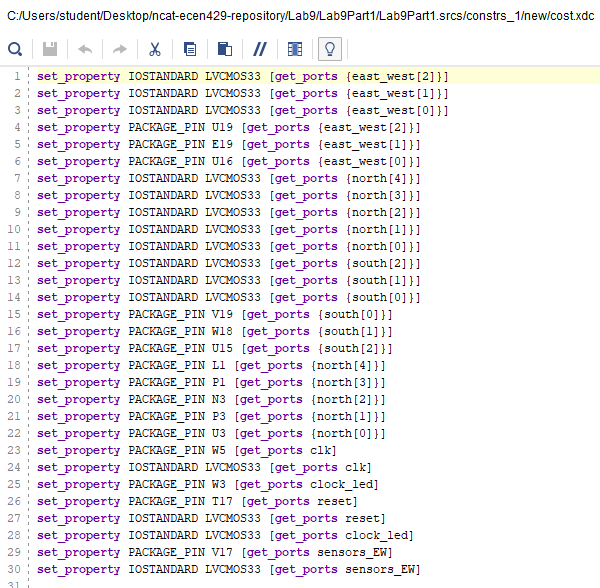
\includegraphics[scale=1]{./images/Part1/l9p1const.png}
	\caption{\label{fig:Prob1Const}Constraints file for Problem 1.}
\end{figure}
\end{center}

\section{Problem 2 VHDL Code}
\begin{lstlisting}[language=VHDL]
library IEEE;
use IEEE.STD_LOGIC_1164.ALL;

entity Lab9Part2 is
    Port ( clk : in STD_LOGIC;
           reset : in STD_LOGIC;
           sensors_EW : in STD_LOGIC_VECTOR(1 downto 0);
           sensor_NT : in STD_LOGIC;
           north : out STD_LOGIC_VECTOR(4 downto 0);
           south : out STD_LOGIC_VECTOR(2 downto 0);
           east_west : out STD_LOGIC_VECTOR(2 downto 0);
           clock_led : out STD_LOGIC);
end Lab9Part2;

architecture Behavioral of Lab9Part2 is

component clock_divider is
     port(clk : in std_logic;
          start_timer : in std_logic;
	  FastClock,MediumClock,SlowClock, led0 : out std_logic);
end component clock_divider;

signal current_state : STD_LOGIC_VECTOR(3 downto 0) := "0000";
signal next_state : STD_LOGIC_VECTOR(3 downto 0) := "0000";
signal start_timer : STD_LOGIC := '0';
signal fast_clock : STD_LOGIC;
signal medium_clock : STD_LOGIC;
signal slow_clock : STD_LOGIC;

begin
    clk_div : clock_divider port map(clk, start_timer, fast_clock, medium_clock, slow_clock, clock_led);
    
    process(slow_clock, reset)
    begin
        if(reset = '1') then next_state <= "0000";
        elsif(slow_clock'event and slow_clock = '1') then
            case current_state is
                when "0000" =>
                    if(sensors_EW = "01" or sensors_EW = "10" or sensors_EW = "11") then
                        next_state <= "0001";
                    elsif(sensor_NT = '1') then 
                        next_state <= "0111";
                    else
                        next_state <= "0000";
                    end if;
                when "0001" =>
                    next_state <= "0010";
                when "0010" =>
                    next_state <= "0011";
                when "0011" =>
                    if(sensors_EW = "01" or sensors_EW = "10" or sensors_EW = "11") then
                        next_state <= "0011";
                    else
                        next_state <= "0100";
                    end if;
                when "0100" =>
                    next_state <= "0101";
                when "0101" =>
                    if(sensor_NT = '1') then
                        next_state <= "0110";
                    else
                        next_state <= "0000";
                    end if;
                when "0110" =>
                    if(sensor_NT = '1') then
                        next_state <= "0110";
                    else
                        next_state <= "1001";
                    end if;
                when "0111" =>
                    next_state <= "1000";
                when "1000" =>
                    next_state <= "0110";
                when "1001" =>
                    next_state <= "1010";
                when others =>
                    next_state <= "0000";
            end case;
        end if;
    end process;
    process(current_state)
    begin
        case current_state is
            when "0000" =>
                north <= "00001";
                south <= "001";
                east_west <= "100";
            when "0001" =>
                north <= "01000";
                south <= "010";
                east_west <= "100";
            when "0010" =>
                north <= "10000";
                south <= "100";
                east_west <= "100";
            when "0011" =>
                north <= "10000";
                south <= "100";
                east_west <= "001";
            when "0100" =>
                north <= "10000";
                south <= "100";
                east_west <= "010";
            when "0101" =>
                north <= "10000";
                south <= "100";
                east_west <= "100";
            when "0110" =>
                north <= "00011";
                south <= "100";
                east_west <= "100";
            when "0111" =>
                north <= "00001";
                south <= "010";
                east_west <= "100";
            when "1000" =>
                north <= "00001";
                south <= "100";
                east_west <= "100";
            when "1001" =>
                north <= "00101";
                south <= "100";
                east_west <= "100";
            when others =>
                north <= "00001";
                south <= "100";
                east_west <= "100";
        end case;
    end process;
    current_state <= next_state;
end Behavioral;
\end{lstlisting}

\section{Problem 2 Constraints File}
\begin{center}
\begin{figure}[H]
	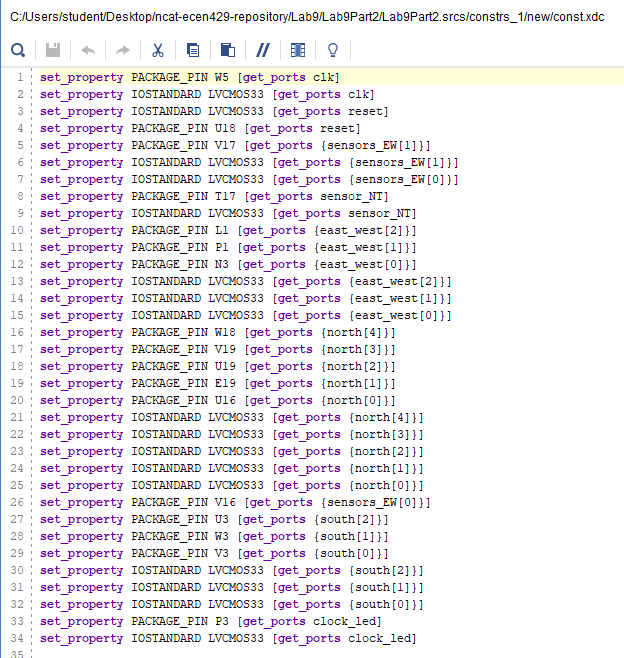
\includegraphics[scale=1]{./images/Part2/l9p2const.png}
	\caption{\label{fig:Prob2Const}Constraints file for Problem 2.}
\end{figure}
\end{center}

\section{Problem 3 VHDL Code}
\begin{lstlisting}[language=VHDL]
library IEEE;
use IEEE.STD_LOGIC_1164.ALL;

entity traffic_control is
    Port ( clk : in STD_LOGIC;
           reset : in STD_LOGIC;
           sensors_EW : in STD_LOGIC_VECTOR(1 downto 0);
           sensor_NT : in STD_LOGIC;
           north : out STD_LOGIC_VECTOR(4 downto 0);
           south : out STD_LOGIC_VECTOR(2 downto 0);
           east_west : out STD_LOGIC_VECTOR(2 downto 0);
           clock_led : out STD_LOGIC;
           output_count : out STD_LOGIC_VECTOR(6 downto 0);
           output_mux : out STD_LOGIC_VECTOR(3 downto 0));
end traffic_control;

architecture Behavioral of traffic_control is

component clock_divider is
     port(clk : in std_logic;
          start_timer : in std_logic;
	  FastClock,MediumClock,SlowClock, led0 : out std_logic);
end component clock_divider;

component traffic_count is
    port(clk, e_signal, w_signal : in STD_LOGIC;
        nt_signal : in STD_LOGIC;
        output_count : out STD_LOGIC_VECTOR(6 downto 0);
        output_mux : out STD_LOGIC_VECTOR(3 downto 0));
end component traffic_count;

signal current_state : STD_LOGIC_VECTOR(3 downto 0) := "0000";
signal next_state : STD_LOGIC_VECTOR(3 downto 0) := "0000";
signal start_timer : STD_LOGIC := '0';
signal fast_clock : STD_LOGIC;
signal medium_clock : STD_LOGIC;
signal slow_clock : STD_LOGIC;
signal sig_count : STD_LOGIC_VECTOR(6 downto 0);
signal sig_mux : STD_LOGIC_VECTOR(3 downto 0);

begin
    clk_div : clock_divider port map(clk, start_timer, fast_clock, medium_clock, slow_clock, clock_led);
    traf_cnt : traffic_count port map(fast_clock, sensors_EW(0), sensors_EW(1), sensor_NT, sig_count, sig_mux);
    
    process(slow_clock, reset)
    begin
        if(reset = '1') then next_state <= "0000";
        elsif(slow_clock'event and slow_clock = '1') then
            case current_state is
                when "0000" =>
                    if(sensors_EW = "01" or sensors_EW = "10" or sensors_EW = "11") then
                        next_state <= "0001";
                    elsif(sensor_NT = '1') then 
                        next_state <= "0111";
                    else
                        next_state <= "0000";
                    end if;
                when "0001" =>
                    next_state <= "0010";
                when "0010" =>
                    next_state <= "0011";
                when "0011" =>
                    if(sensors_EW = "01" or sensors_EW = "10" or sensors_EW = "11") then
                        next_state <= "0011";
                    else
                        next_state <= "0100";
                    end if;
                when "0100" =>
                    next_state <= "0101";
                when "0101" =>
                    if(sensor_NT = '1') then
                        next_state <= "0110";
                    else
                        next_state <= "0000";
                    end if;
                when "0110" =>
                    if(sensor_NT = '1') then
                        next_state <= "0110";
                    else
                        next_state <= "1001";
                    end if;
                when "0111" =>
                    next_state <= "1000";
                when "1000" =>
                    next_state <= "0110";
                when "1001" =>
                    next_state <= "1010";
                when others =>
                    next_state <= "0000";
            end case;
        end if;
    end process;
    process(current_state)
    begin
        case current_state is
            when "0000" =>
                north <= "00001";
                south <= "001";
                east_west <= "100";
            when "0001" =>
                north <= "01000";
                south <= "010";
                east_west <= "100";
            when "0010" =>
                north <= "10000";
                south <= "100";
                east_west <= "100";
            when "0011" =>
                north <= "10000";
                south <= "100";
                east_west <= "001";
            when "0100" =>
                north <= "10000";
                south <= "100";
                east_west <= "010";
            when "0101" =>
                north <= "10000";
                south <= "100";
                east_west <= "100";
            when "0110" =>
                north <= "00011";
                south <= "100";
                east_west <= "100";
            when "0111" =>
                north <= "00001";
                south <= "010";
                east_west <= "100";
            when "1000" =>
                north <= "00001";
                south <= "100";
                east_west <= "100";
            when "1001" =>
                north <= "00101";
                south <= "100";
                east_west <= "100";
            when others =>
                north <= "00001";
                south <= "100";
                east_west <= "100";
        end case;
    end process;
    current_state <= next_state;
    output_count <= sig_count;
    output_mux <= sig_mux;
end Behavioral;


library IEEE;
use IEEE.STD_LOGIC_1164.ALL;
use IEEE.NUMERIC_STD.ALL;

entity traffic_count is
    port(clk, e_signal, w_signal : in STD_LOGIC;
    nt_signal : in STD_LOGIC;
    output_count : out STD_LOGIC_VECTOR(6 downto 0);
    output_mux : out STD_LOGIC_VECTOR(3 downto 0));
end entity traffic_count;

architecture Behavioral of traffic_count is
signal ew_count : STD_LOGIC_VECTOR(3 downto 0) := "0000";
signal nt_count : STD_LOGIC_VECTOR(3 downto 0) := "0000";

begin
    process(e_signal, w_signal)
    begin
        if(e_signal = '1' or w_signal = '1') then ew_count <= STD_LOGIC_VECTOR(to_unsigned(to_integer(unsigned(ew_count)) + 1, 4));
        end if;
    end process;
    process(nt_signal)
    begin
        if(nt_signal = '1') then nt_count <= STD_LOGIC_VECTOR(to_unsigned(to_integer(unsigned(ew_count)) + 1, 4));
        end if;
    end process;
    
    process(ew_count, nt_count)
    begin
        output_mux <= "0001";
        case ew_count is
            when "0000" =>
                output_count <= "0000001";
            when "0001" =>
                output_count <= "1001111";
            when "0010" =>
                output_count <= "0010010";
            when "0011" =>
                output_count <= "0000110";
            when "0100" =>
                output_count <= "1001100";
            when "0101" =>
                output_count <= "0100100";
            when "0110" =>
                output_count <= "0100000";
            when "0111" =>
                output_count <= "0001111";
            when "1000" =>
                output_count <= "0000000";
            when "1001" =>
                output_count <= "0001100";
            when others =>
                output_count <= "1111111";
        end case;
        output_mux <= "0100";
        case nt_count is
            when "0000" =>
                output_count <= "0000001";
            when "0001" =>
                output_count <= "1001111";
            when "0010" =>
                output_count <= "0010010";
            when "0011" =>
                output_count <= "0000110";
            when "0100" =>
                output_count <= "1001100";
            when "0101" =>
                output_count <= "0100100";
            when "0110" =>
                output_count <= "0100000";
            when "0111" =>
                output_count <= "0001111";
            when "1000" =>
                output_count <= "0000000";
            when "1001" =>
                output_count <= "0001100";
            when others =>
                output_count <= "1111111";
        end case;
    end process;
end Behavioral;
\end{lstlisting}

\section{Problem 3 Constraints File}
\begin{center}
\begin{figure}[H]
	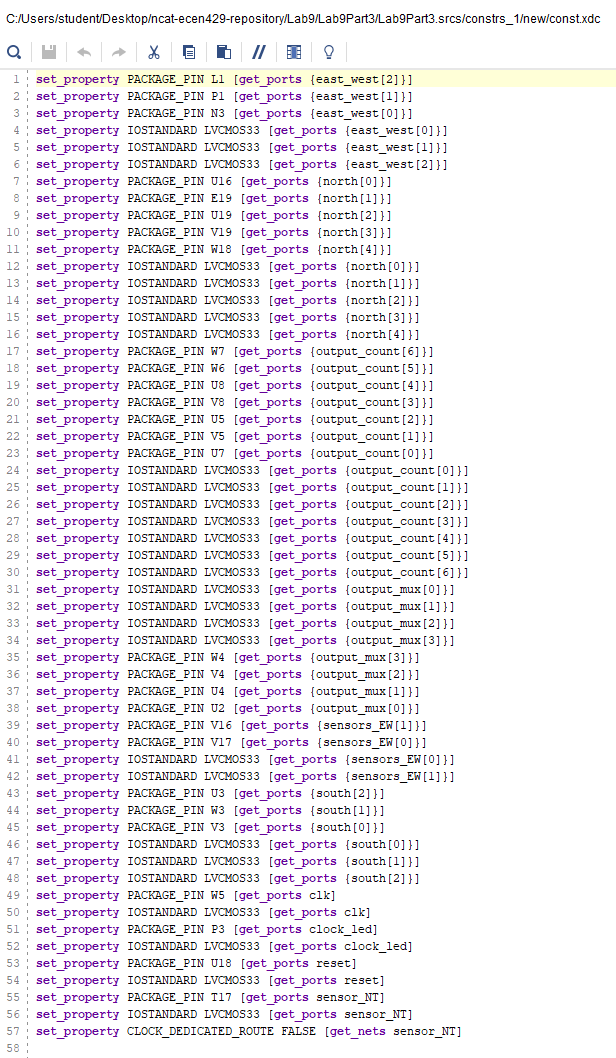
\includegraphics[scale=0.7]{./images/l9p3const.png}
	\caption{\label{fig:Prob3Const}Constraints file for Problem 3.}
\end{figure}
\end{center}

\end{appendices}
\end{document}
